\documentclass[a4paper,11pt]{article}
\usepackage[margin=1in]{geometry}
\usepackage{polski}
\usepackage{upgreek}
\usepackage{booktabs}
\usepackage[utf8]{inputenc}
\frenchspacing
\usepackage{enumerate}
\usepackage{graphicx}

\usepackage{tabularx}

\usepackage{listings} % do wstawienia kodu
\usepackage{xcolor} % do wstawienia kodu
\lstset { %
    language=C++,
    backgroundcolor=\color{black!5}, % set backgroundcolor
    basicstyle=\footnotesize,% basic font setting
    breaklines=true,                 % sets automatic line breaking
    backgroundcolor=\color{white},
    numbers=left,
    frame=single,
}

\usepackage{pstricks-add} % do definicji
\usepackage{float} % do obrazków
\usepackage{hyperref} % linki
% kilka definicji
\graphicspath{{./images/}}
\def\SCALE{0.6}
\hypersetup{ % coby ładnie wyglądało
    colorlinks,
    citecolor=black,
    filecolor=black,
    linkcolor=black,
    urlcolor=black
}
\begin{document}
\title{DTR Pszemeg}

\maketitle

\begin{center}
\begin{figure}[H]
	\centering
	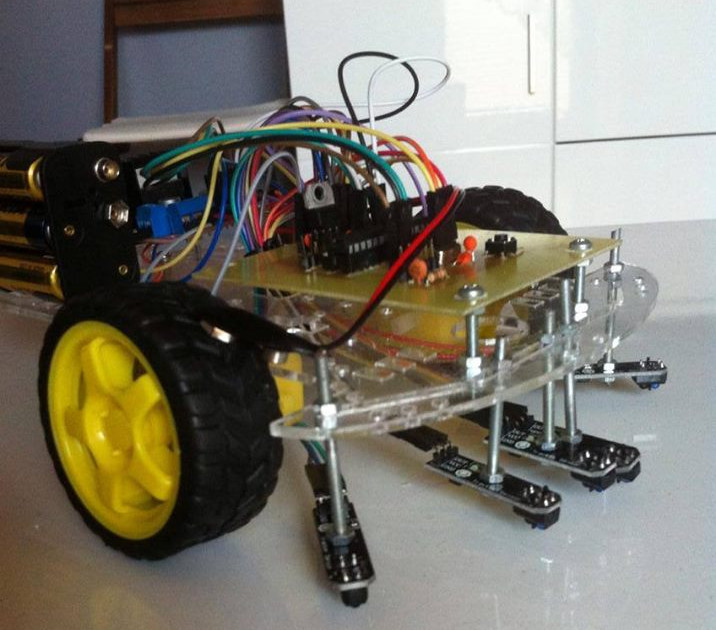
\includegraphics[width=\SCALE
	\paperwidth]{Pszemeg}
	\caption{Pszemeg}
\end{figure}

\begin{tabularx}{\textwidth}{|l|l|X|}
\hline
imie		& nazwisko		& przydział zadań \\ \hline
Piotr	& Binkowski		& zamawianie i kompletowanie podzespołów, projekt płytki drukowanej, nadzorowanie prac			\\
Adam		& Ćwian			& wytrawianie płytki (termotransfer)			\\
Paweł	& Miłończyk		& DTR, lutowanie płytki, trawienie płytki, wykonanie termometru odpornego na wrzątek			\\
Juliusz & Sałek			& kapitan, wykonanie tras, DTR, fotorelacja, kąpiel płytki w roztworze			\\
Patryk	& Scheffler		&			\\
Jakub	& Stańczak		& zaprogramowanie robota, wiercenie i czyszczenie płytki, system regulacji czujników			\\
Jorge	& Abreau			& słuchanie i próba zrozumienia dzialania robota i kodu	\\ \hline
\end{tabularx}
\end{center}

\tableofcontents

\listoffigures

\section{Opis}
Celem robota jest podążanie wyznaczoną linią. Jest w stanie pokonywać zakręty do 90$^\circ$ oraz skrzyżowania. Robot najlepiej radzi sobie na łukach, gdyż trzy środkowe czujniki są zbliżone do siebie co umożliwia mu szybkie wprowadzania korekt i płynną jazdę. Problematyczne są ostre zakręty, gdzie linia jest łapana dopiero przez zewnętrzne czujniki. Robot wtedy zwalnia i stara się wrócić na trasę środkowym czujnikiem. W przypadku wypadnięcia z trasy robot będzie wykonywał nawrót w tę stronę, gdzie ostatnio widział linię.

Robot wykorzystuje pięć czujników. Dwa skrajne umieszczone są w znacznym oddaleniu i trochę z tyłu.
Napęd robota wykonany jest z dwóch silników z przekładniami, umieszczonych z przodu pojazdu. Zasilany jest z 6 baterii AA. Czas działania jest szacowany na 2h. Nie zdecydowaliśmy się na zakup akumulatorów, ze względu na wysoki ich koszt oraz wymóg posiadania specjalnej ładowarki. Tym sposobem robot kosztował nas zaledwie ok. 91.20zł.

Niestety, ale duża masa, czujniki położone blisko osi skrętnej oraz gotowe podwozie skutecznie uniemożliwiły nam walkę o dobry czas. Postawiliśmy na dokładność i nasz robot, gdy był ukończony, nigdy nie wypadł z trasy. Wypadanie z trasy było charakterystyczne dla szybkich i małych robotów, które musiały wiele razy startować w eliminacjach by ukończyć trasę.

\section{Elementy}
\subsection{Tabela elementów}

\begin{center}

\begin{tabular}{|l | c|}

	\hline
	nazwa 										& cena			\\ \hline
	2 x silnik 9V z przekładniami i kołami 		& 16,5			\\
	5 x czujnik	TCRT5000 IR						& 9,7			\\
	podwozie										& 30				\\
	mostek h L289N								& 6				\\
	atmega 328P									& 6				\\
	koszyk na 6 baterii							& 4				\\
	wytrawiacz nadsiarczan sodowy b327			& 5,5			\\
	pcb	7x9cm									& 2,5			\\
	4 x kondensator 68nF							& --				\\
	oscylator 16Mhz								& --				\\
	2 x kondensator 22pF							& --				\\
	4 x kondesator 100nF							& --				\\
	stabilizator 7805							& 1				\\
	przycisk monostabilny						& --				\\
	gniazdo dil 28								& 1				\\
	listwa kołkowa jednorzędowa					& --				\\
	śruby i wiertła								& 5				\\
	przewody										& 4				\\
	żelazko										& --				\\
	cyna											& małe ilości	\\
	aceton										& małe ilości	\\
	\hline
\end{tabular}

\end{center}

\subsection{Opis elementów}

\begin{figure}[H]
	\subsubsection{atmega 328P}
		\begin{itemize}
			\item Wyprodukowany przez firmę Atmel.
			\item Obudowa typu dip 28.
			\item Architektura AVR RISC.
			\item Napięcie 1,8V - 5,5V
			\item 8 Mhz na wewnętrznym oscylatorze, możliwość zewnętrznego oscylatora.
		\end{itemize}
	Mikrokontroler jest zgodny z arduino, o ile poprawnie umieszczono oscylator. Jeśli oscylator nie działa mikrokontroler może być dalej zaprogramowany przez	Arduino IDE ale jako atmega 8Mhz.
	
	\centering
	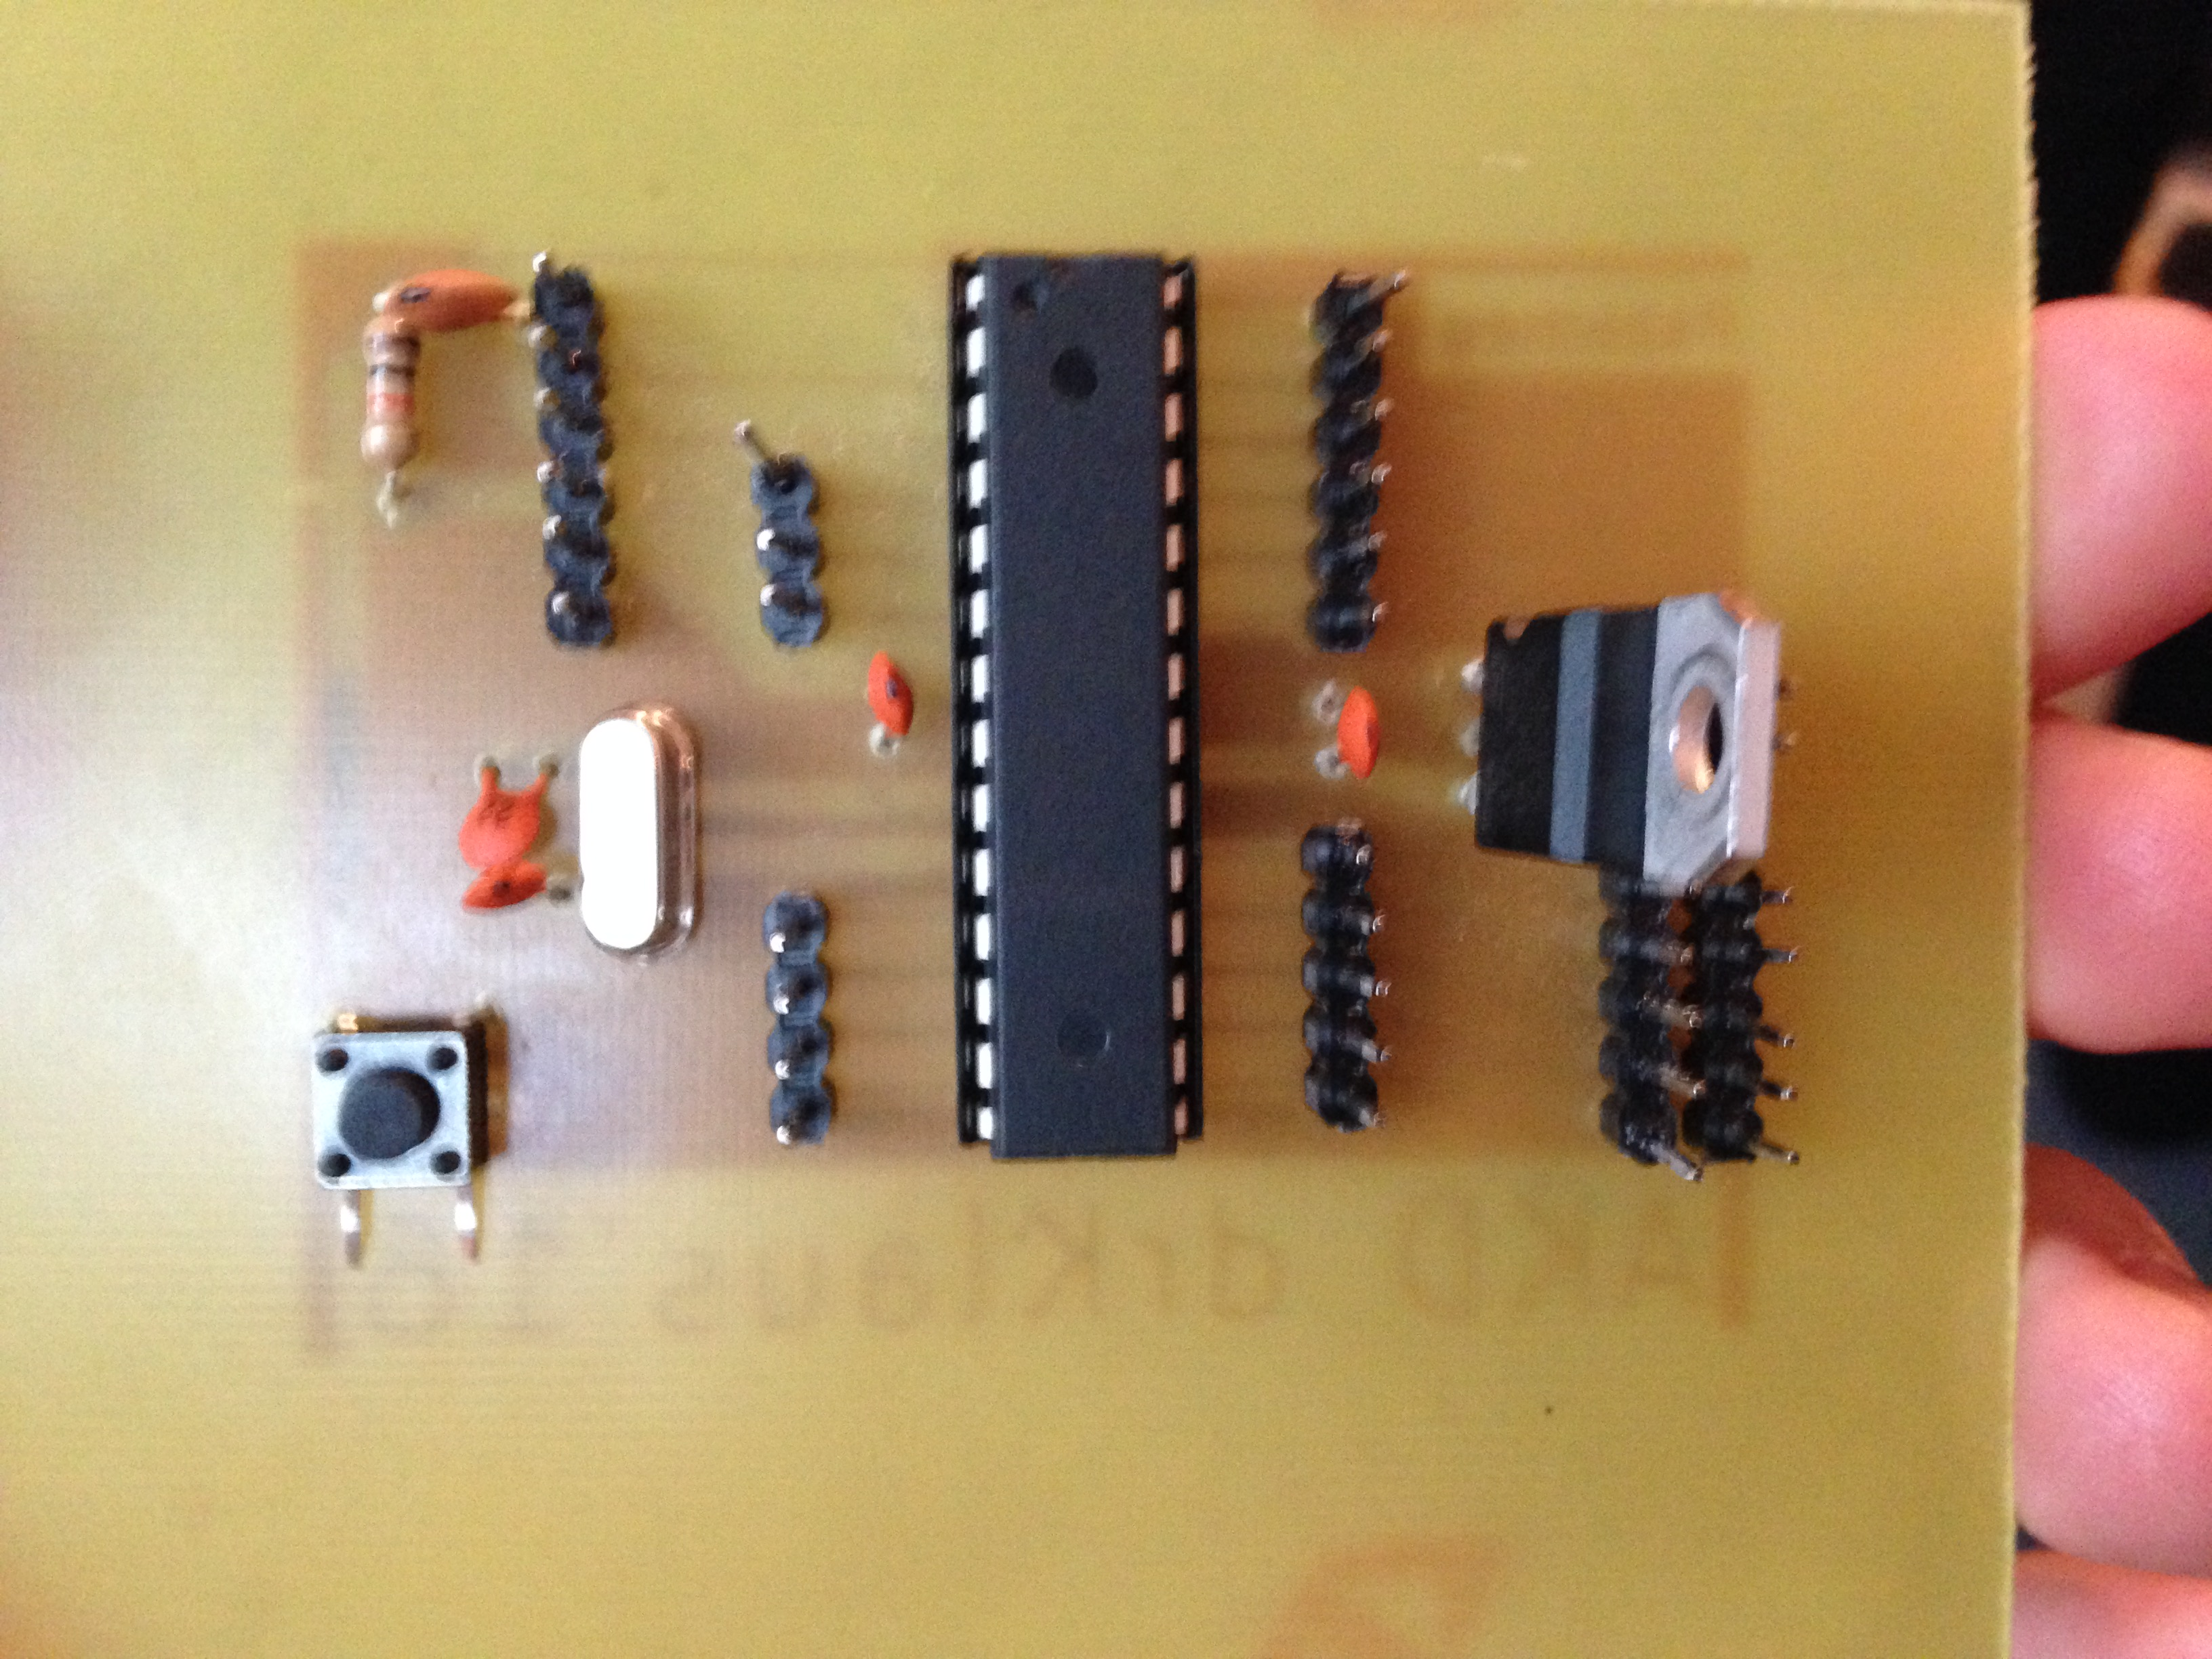
\includegraphics[width=\SCALE
	\paperwidth]{plytkaGotowa}
	\caption{atmega}
	Jest to układ w obudowie DIP, pośrodku zdjęcia.
\end{figure}


\begin{figure}[H]
	\subsubsection{mostek H L298N}
	Do wyjść OUT1 OUT2 należy podłączyć jeden silnik. Do OUT3 i OUT4 drugi. Jeśli silnik kręci się w złą stronę należy odwrócić połączenie.
	Najbardziej skrajne piny (żółte oznaczenie) służą do sterowanie PVM. Czerwone i niebieskie to kierunek obrotów oraz wybór hamulca. Przy podaniu zera na sterowanie PVM nie robi różnicy co poda się na pozostałe, silnik zostanie wyłączony.
	
	\begin{tabular}{|l|l|l|}
		\hline
		LOW & LOW & hamowanie \\
		HIGH & LOW & jazda w przód \\
		LOW & HIGH & jazda w tył \\
		HIGH & HIGH & hamowanie \\
		\hline				
	
	\end{tabular}
	\centering
	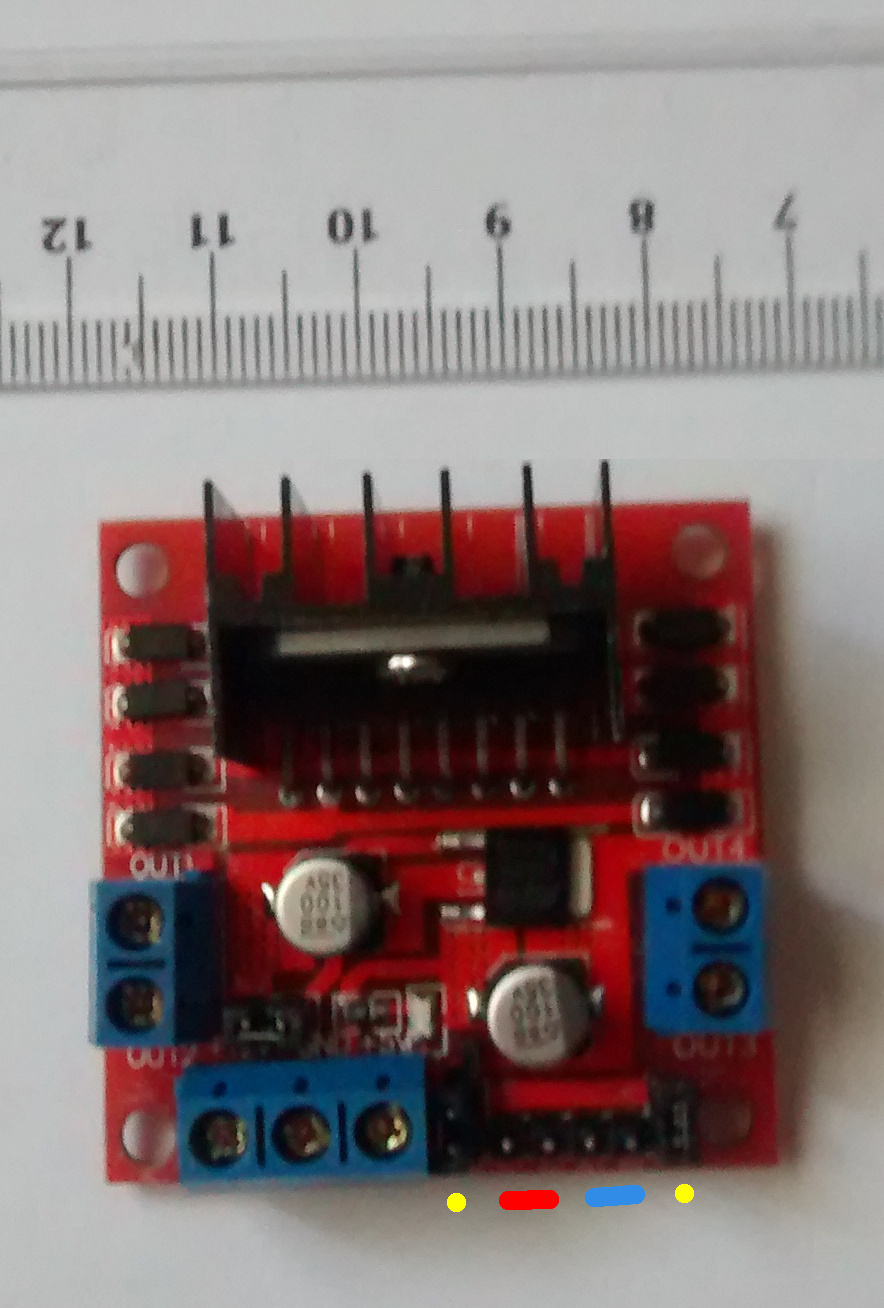
\includegraphics[width=\SCALE
	\paperwidth]{mostek}
	\caption{mostek L298N}
\end{figure}



\begin{figure}[H]
	\subsubsection{silnik}
	\centering
	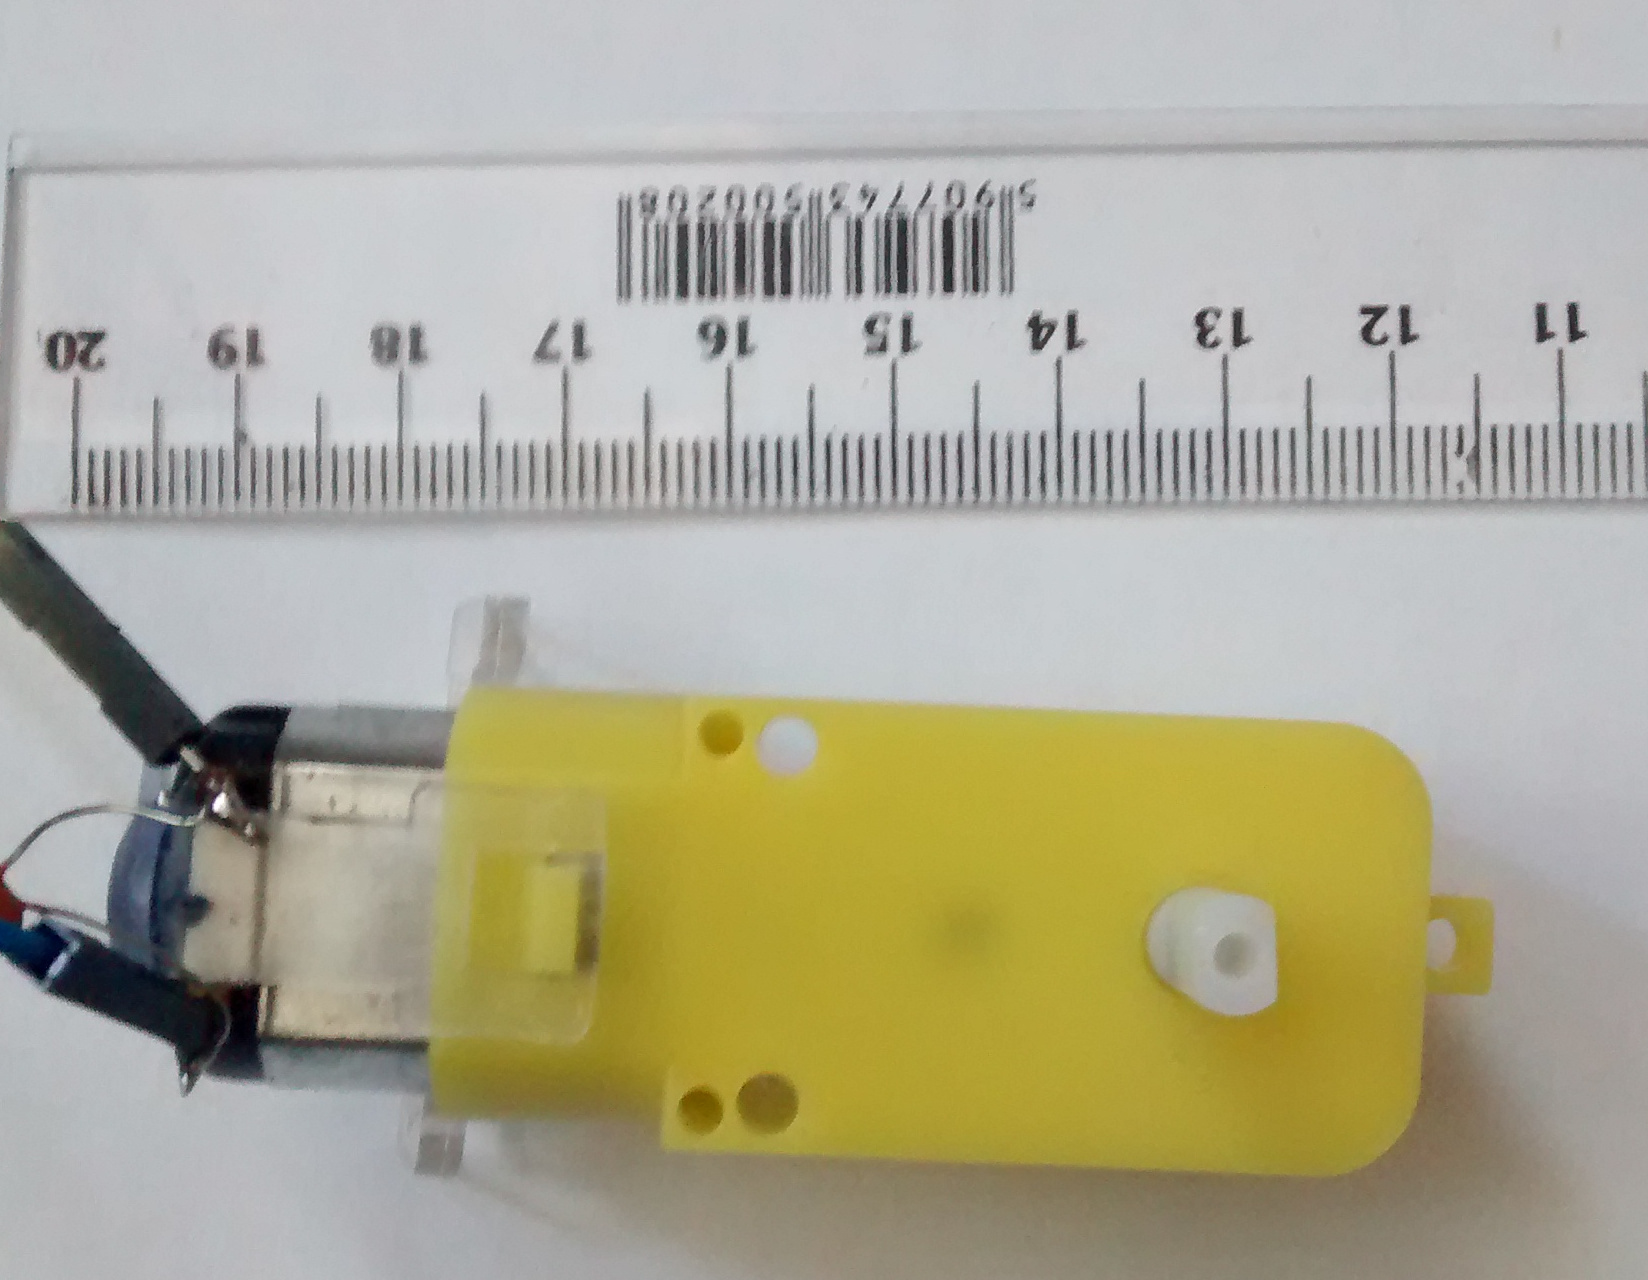
\includegraphics[width=\SCALE
	\paperwidth]{silnik-bok}
	\caption{silnik bok}
	
	\begin{figure}[H]
		\centering
		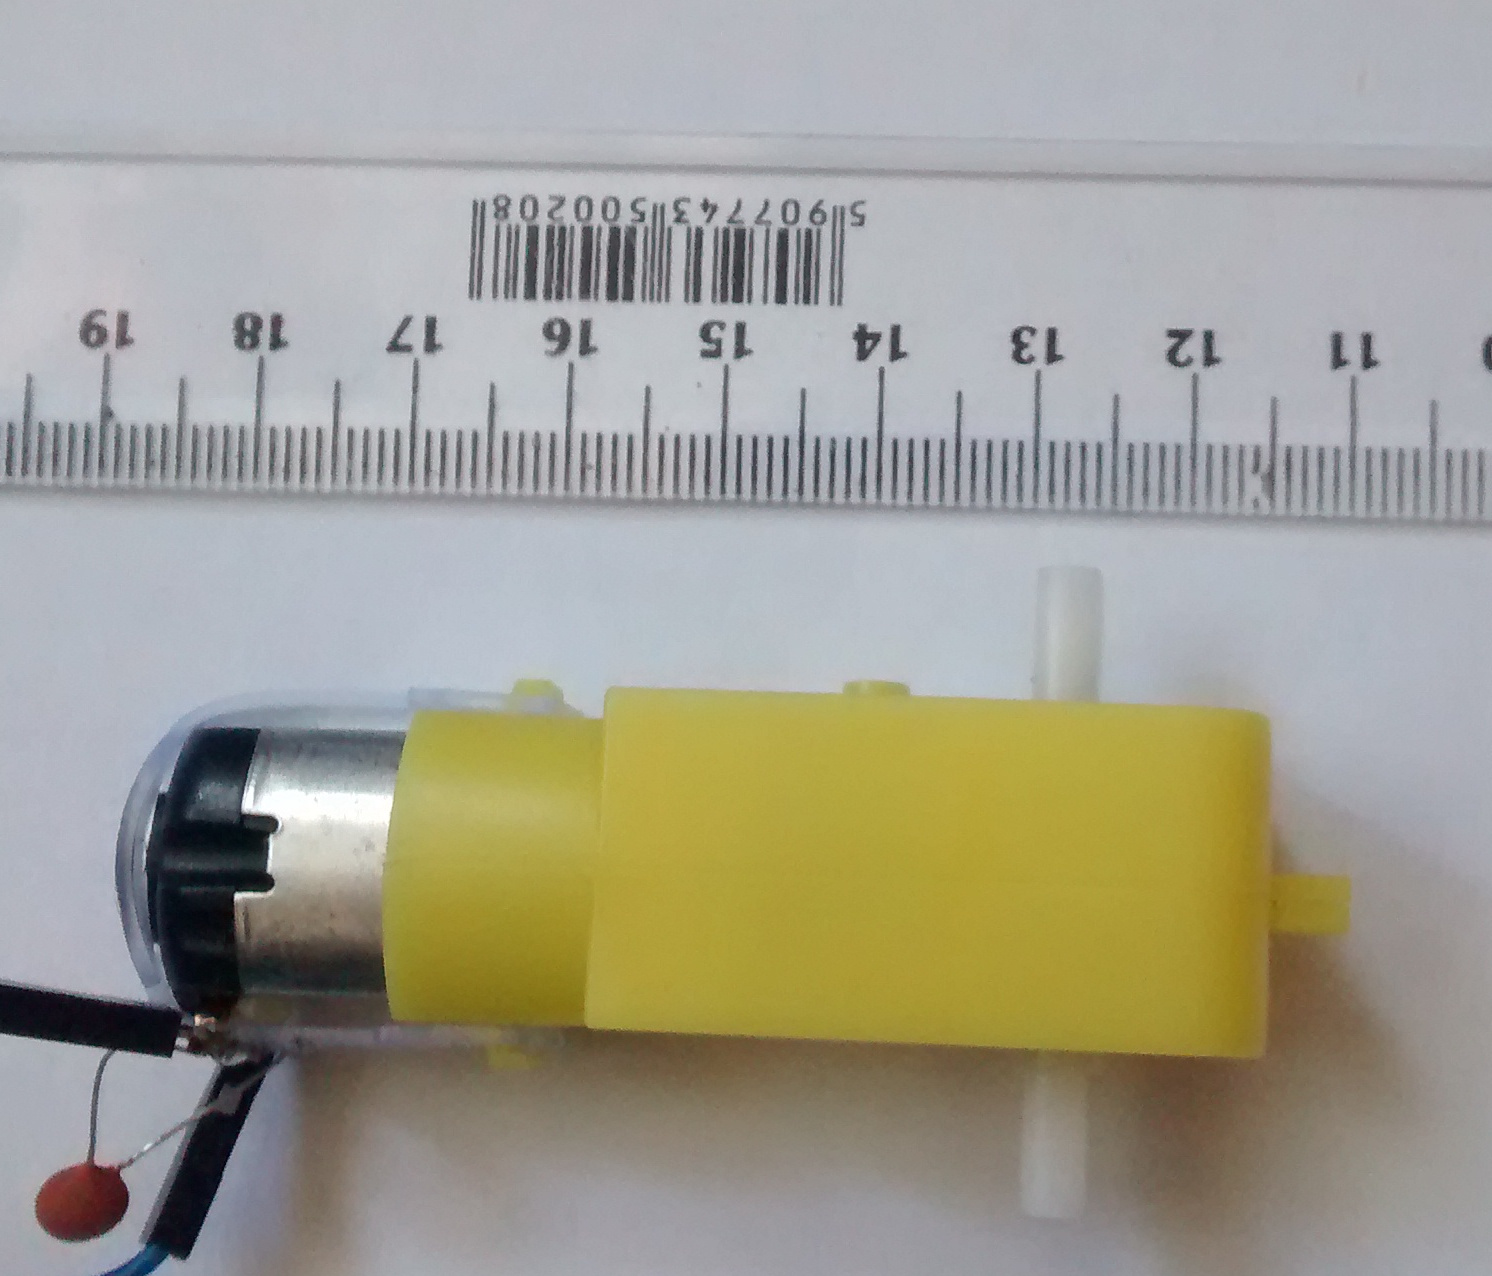
\includegraphics[width=\SCALE
		\paperwidth]{silnik-gora}
		\caption{silnik góra}
	\end{figure}
	
\end{figure}



\begin{figure}[H]
	\subsubsection{zaczepy}
	Przydatne przy mocowaniu silnika, dwa na każdy silnik, po obu stronach mocowane śrubami. W 			podwoziu znajduje się specjalne wycięcie po obu bokach.
	
	\centering
	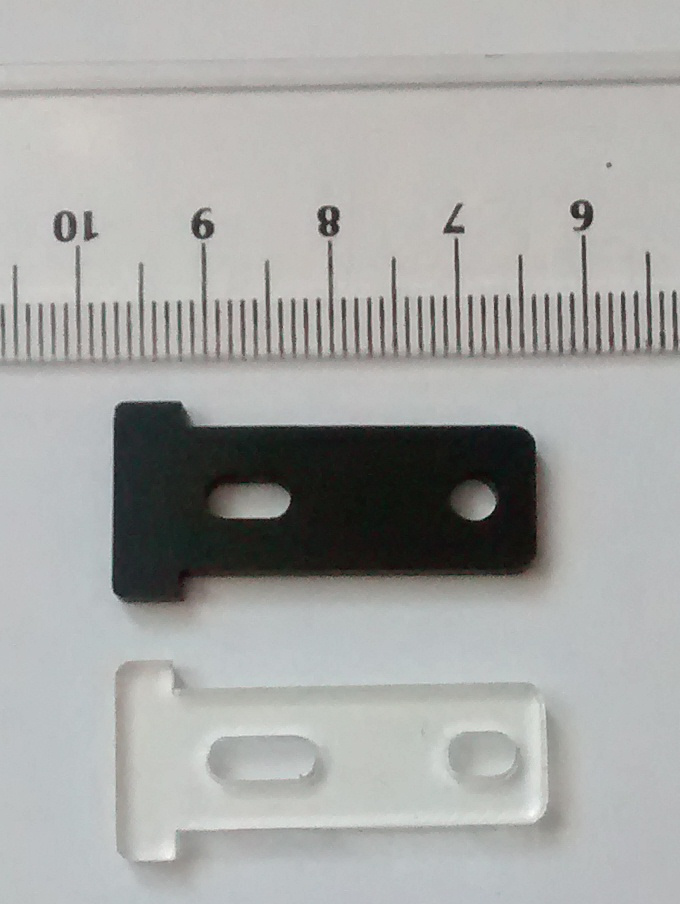
\includegraphics[width=\SCALE
	\paperwidth]{trzymacze}
	\caption{zaczepy}
	

\end{figure}
\begin{figure}[H]
	\centering
	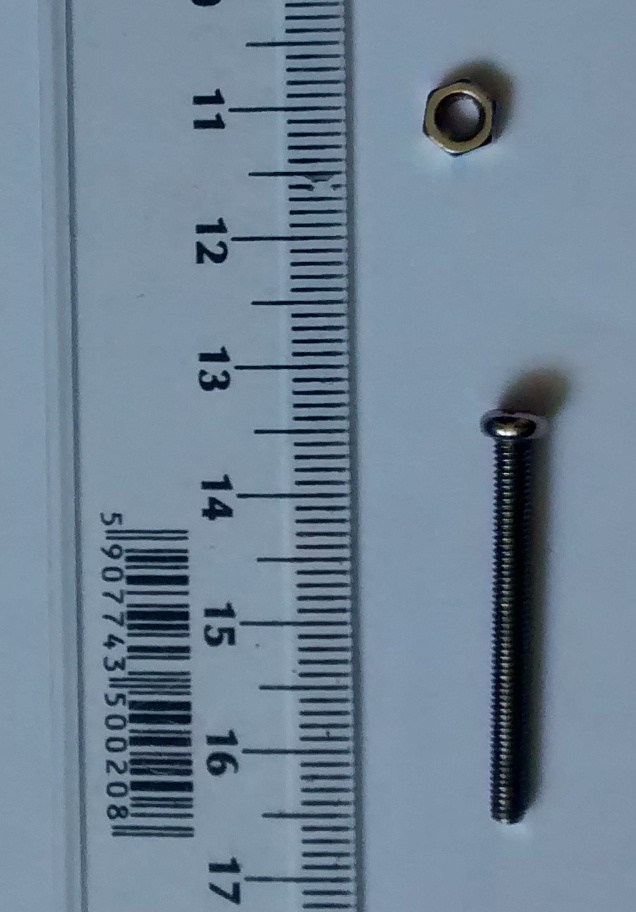
\includegraphics[width=\SCALE
	\paperwidth]{mocowanieSilnika}
	\caption{Mocowanie silnika}
	Śruby którymi łączy się silnik z zaczepami.
\end{figure}	


\begin{figure}[H]
	\subsubsection{koło}
	Należy zwrócić specjalną uwagę, aby koło nie dotykało śruby mocującej.

	\centering
	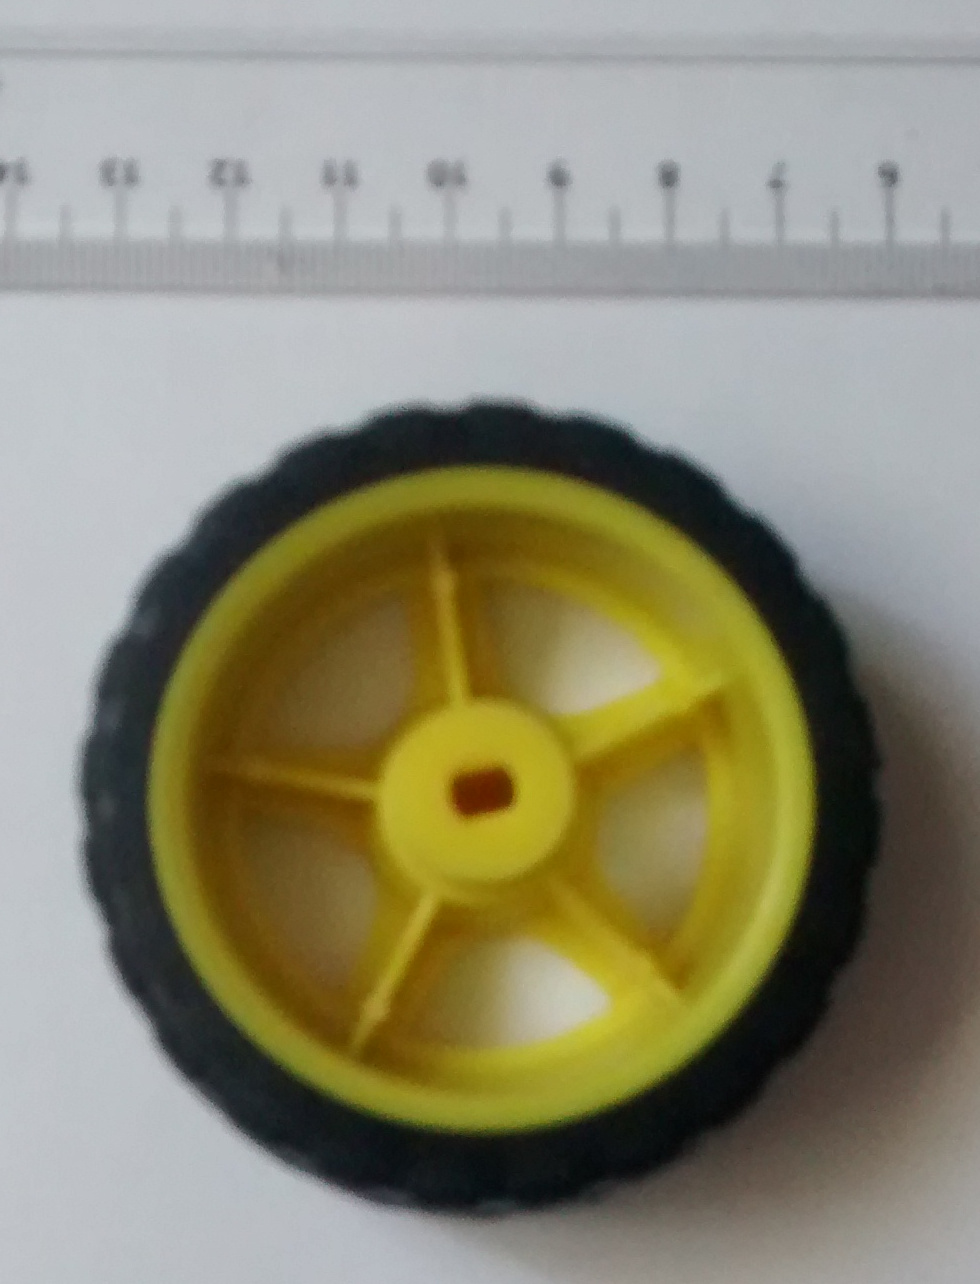
\includegraphics[width=\SCALE
	\paperwidth]{kolo}
	\caption{koło}
\end{figure}

\subsubsection{podstawa}
\begin{figure}[H]
	\centering
	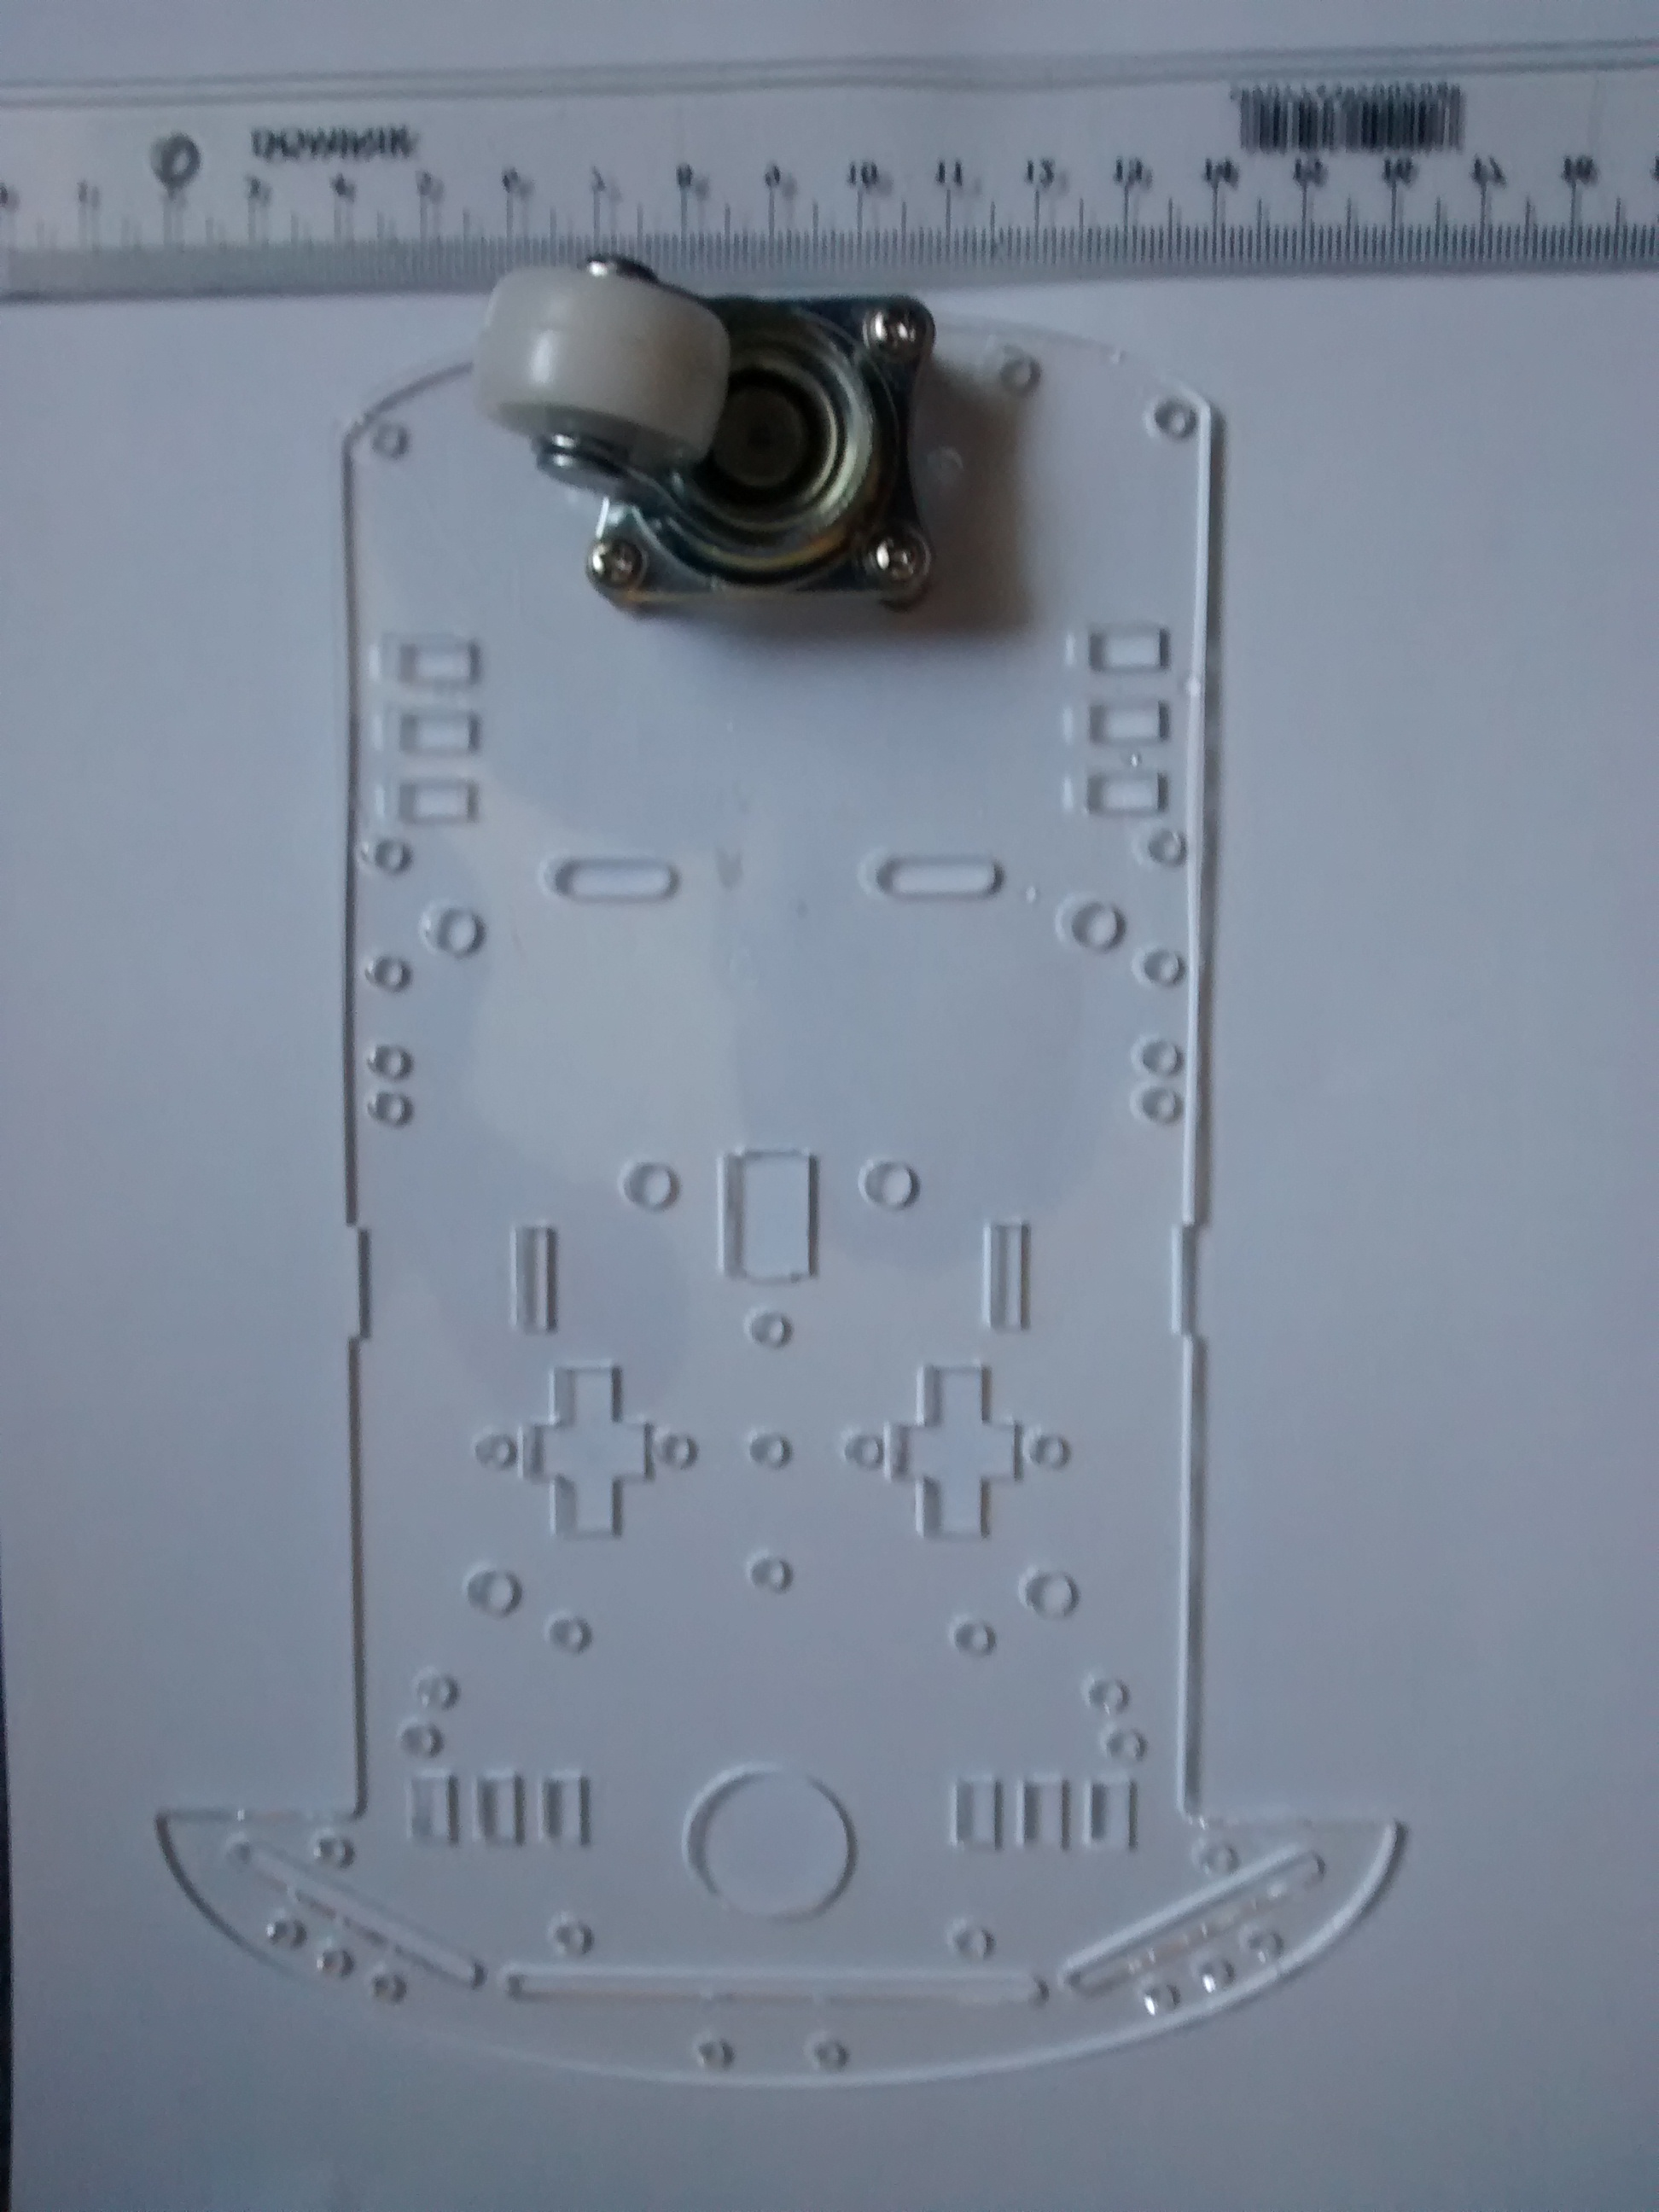
\includegraphics[width=\SCALE
	\paperwidth]{podstawa-1}
	\caption{podstawa}
\end{figure}

\begin{figure}[H]
	\centering
	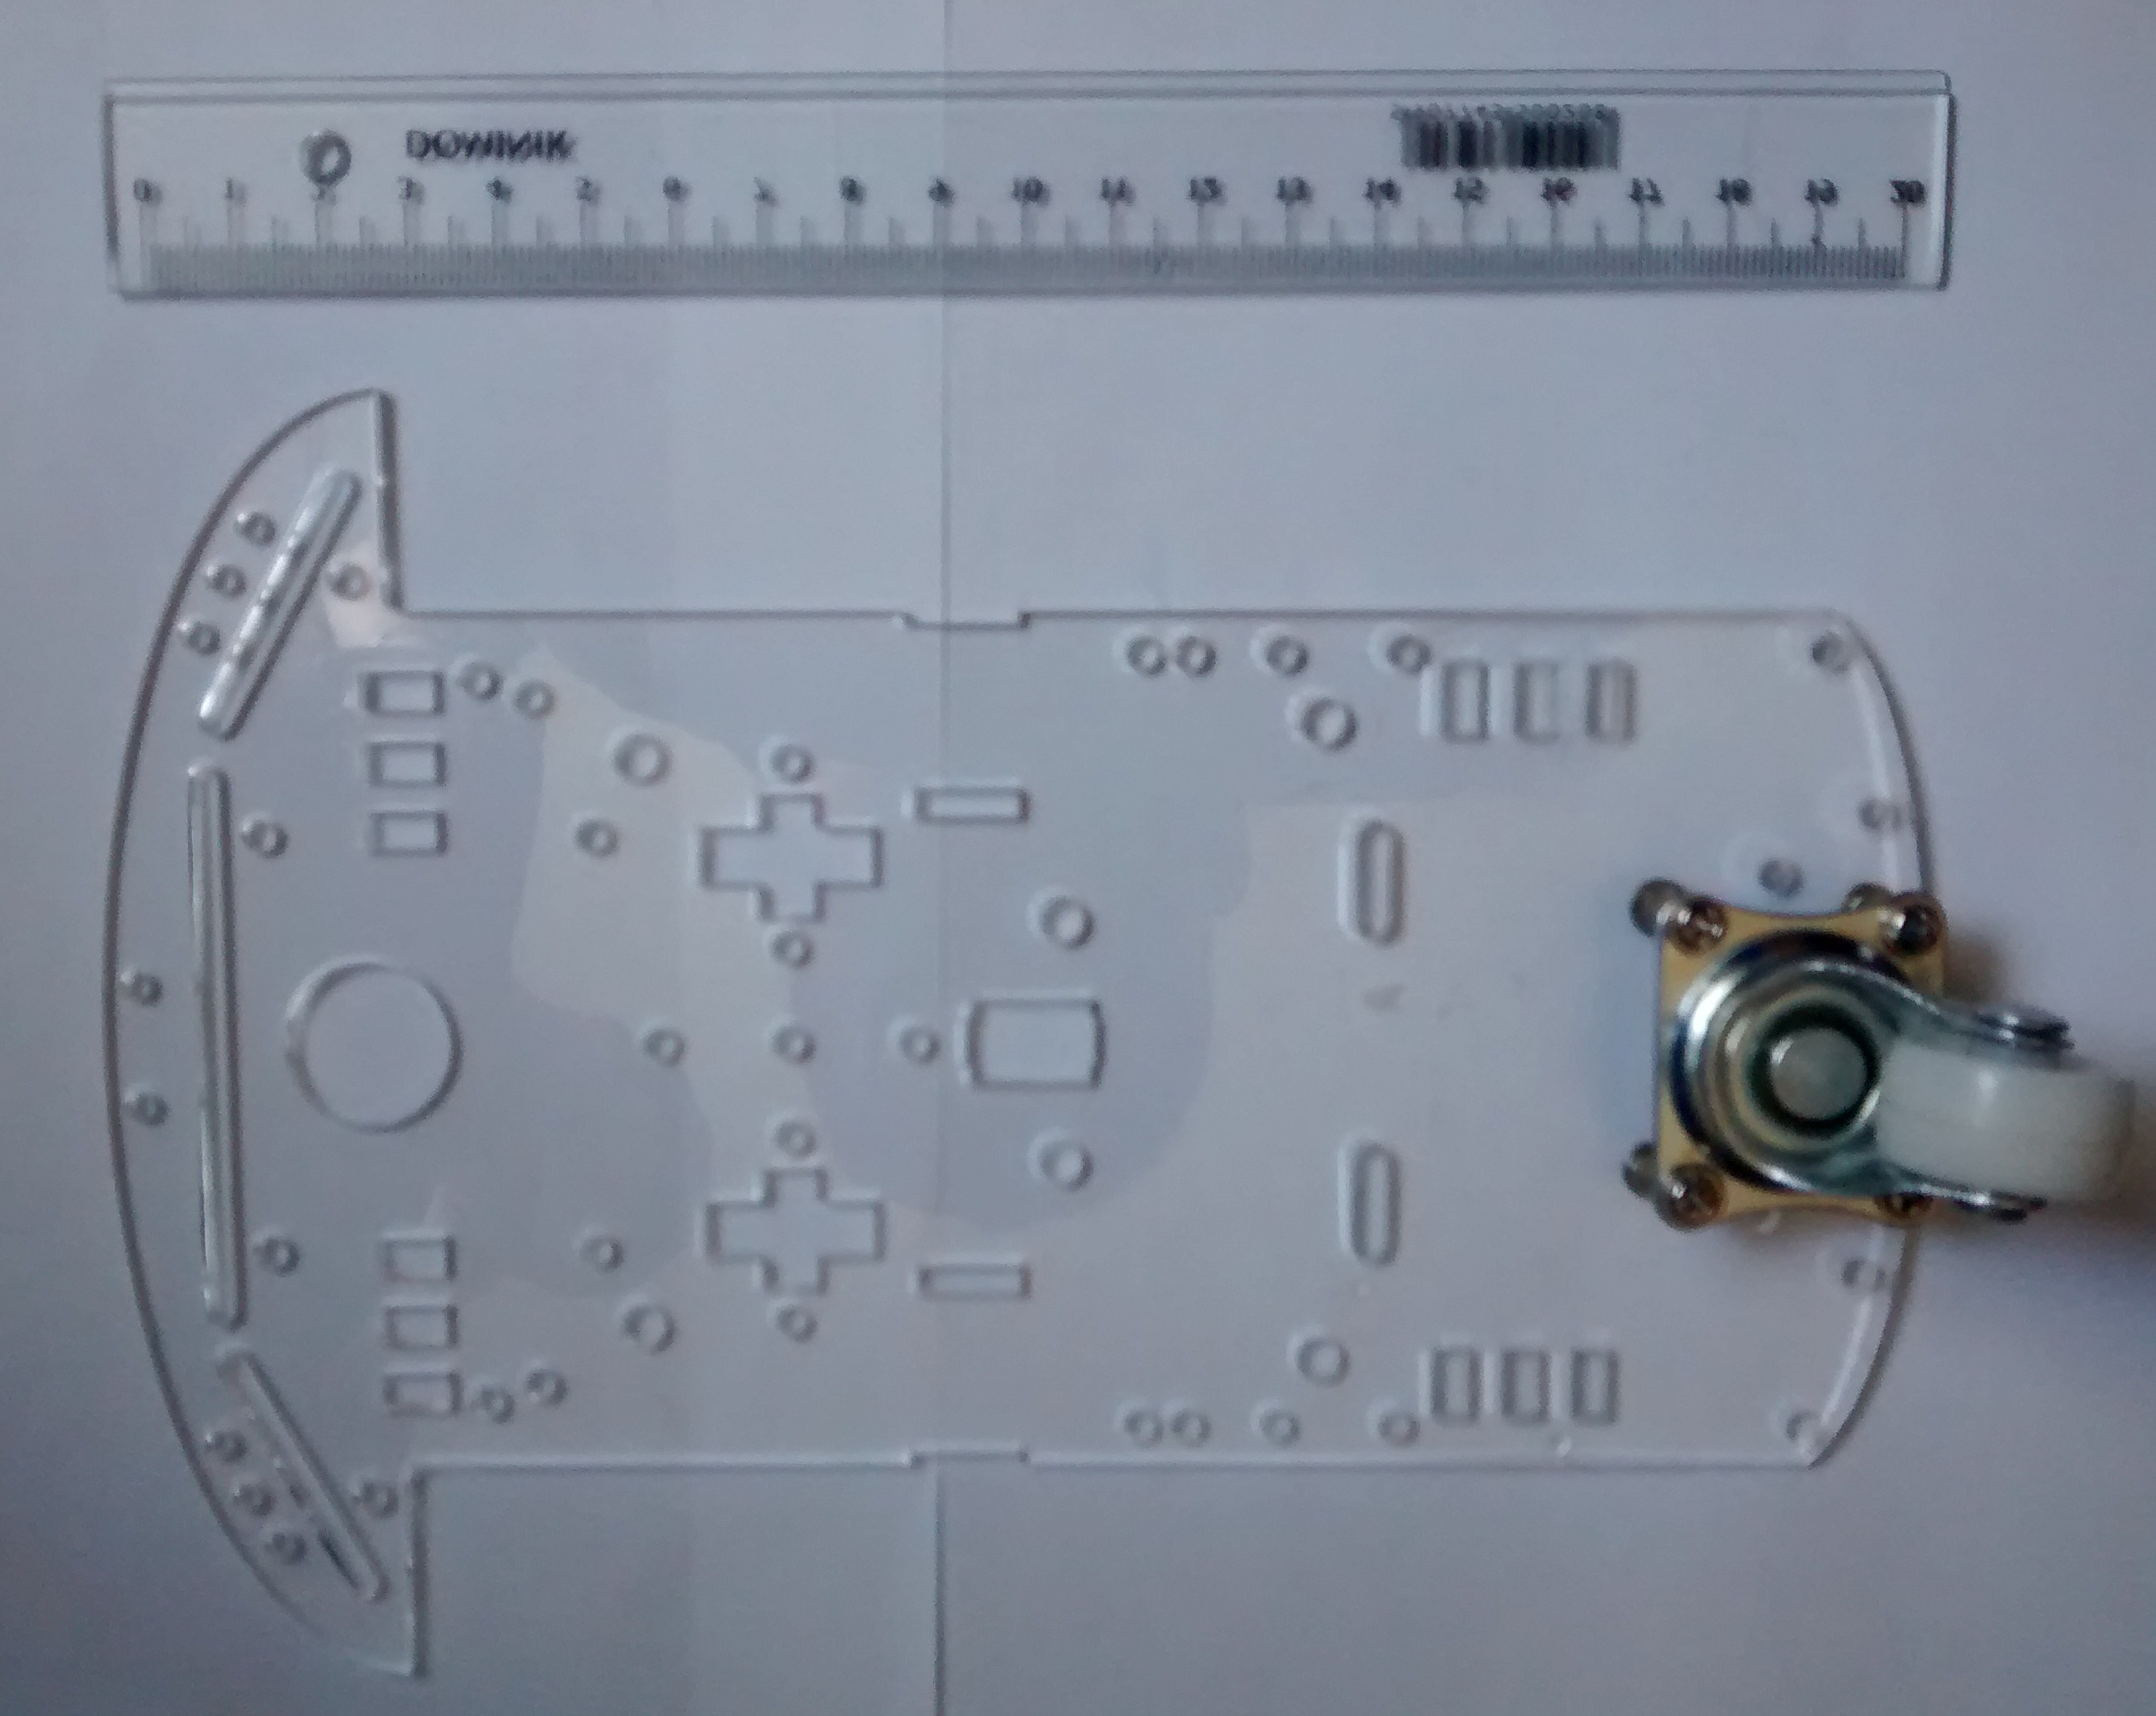
\includegraphics[width=\SCALE
	\paperwidth]{podstawa-2}
	\caption{podstawa}
\end{figure}

\begin{figure}[H]
	\centering
	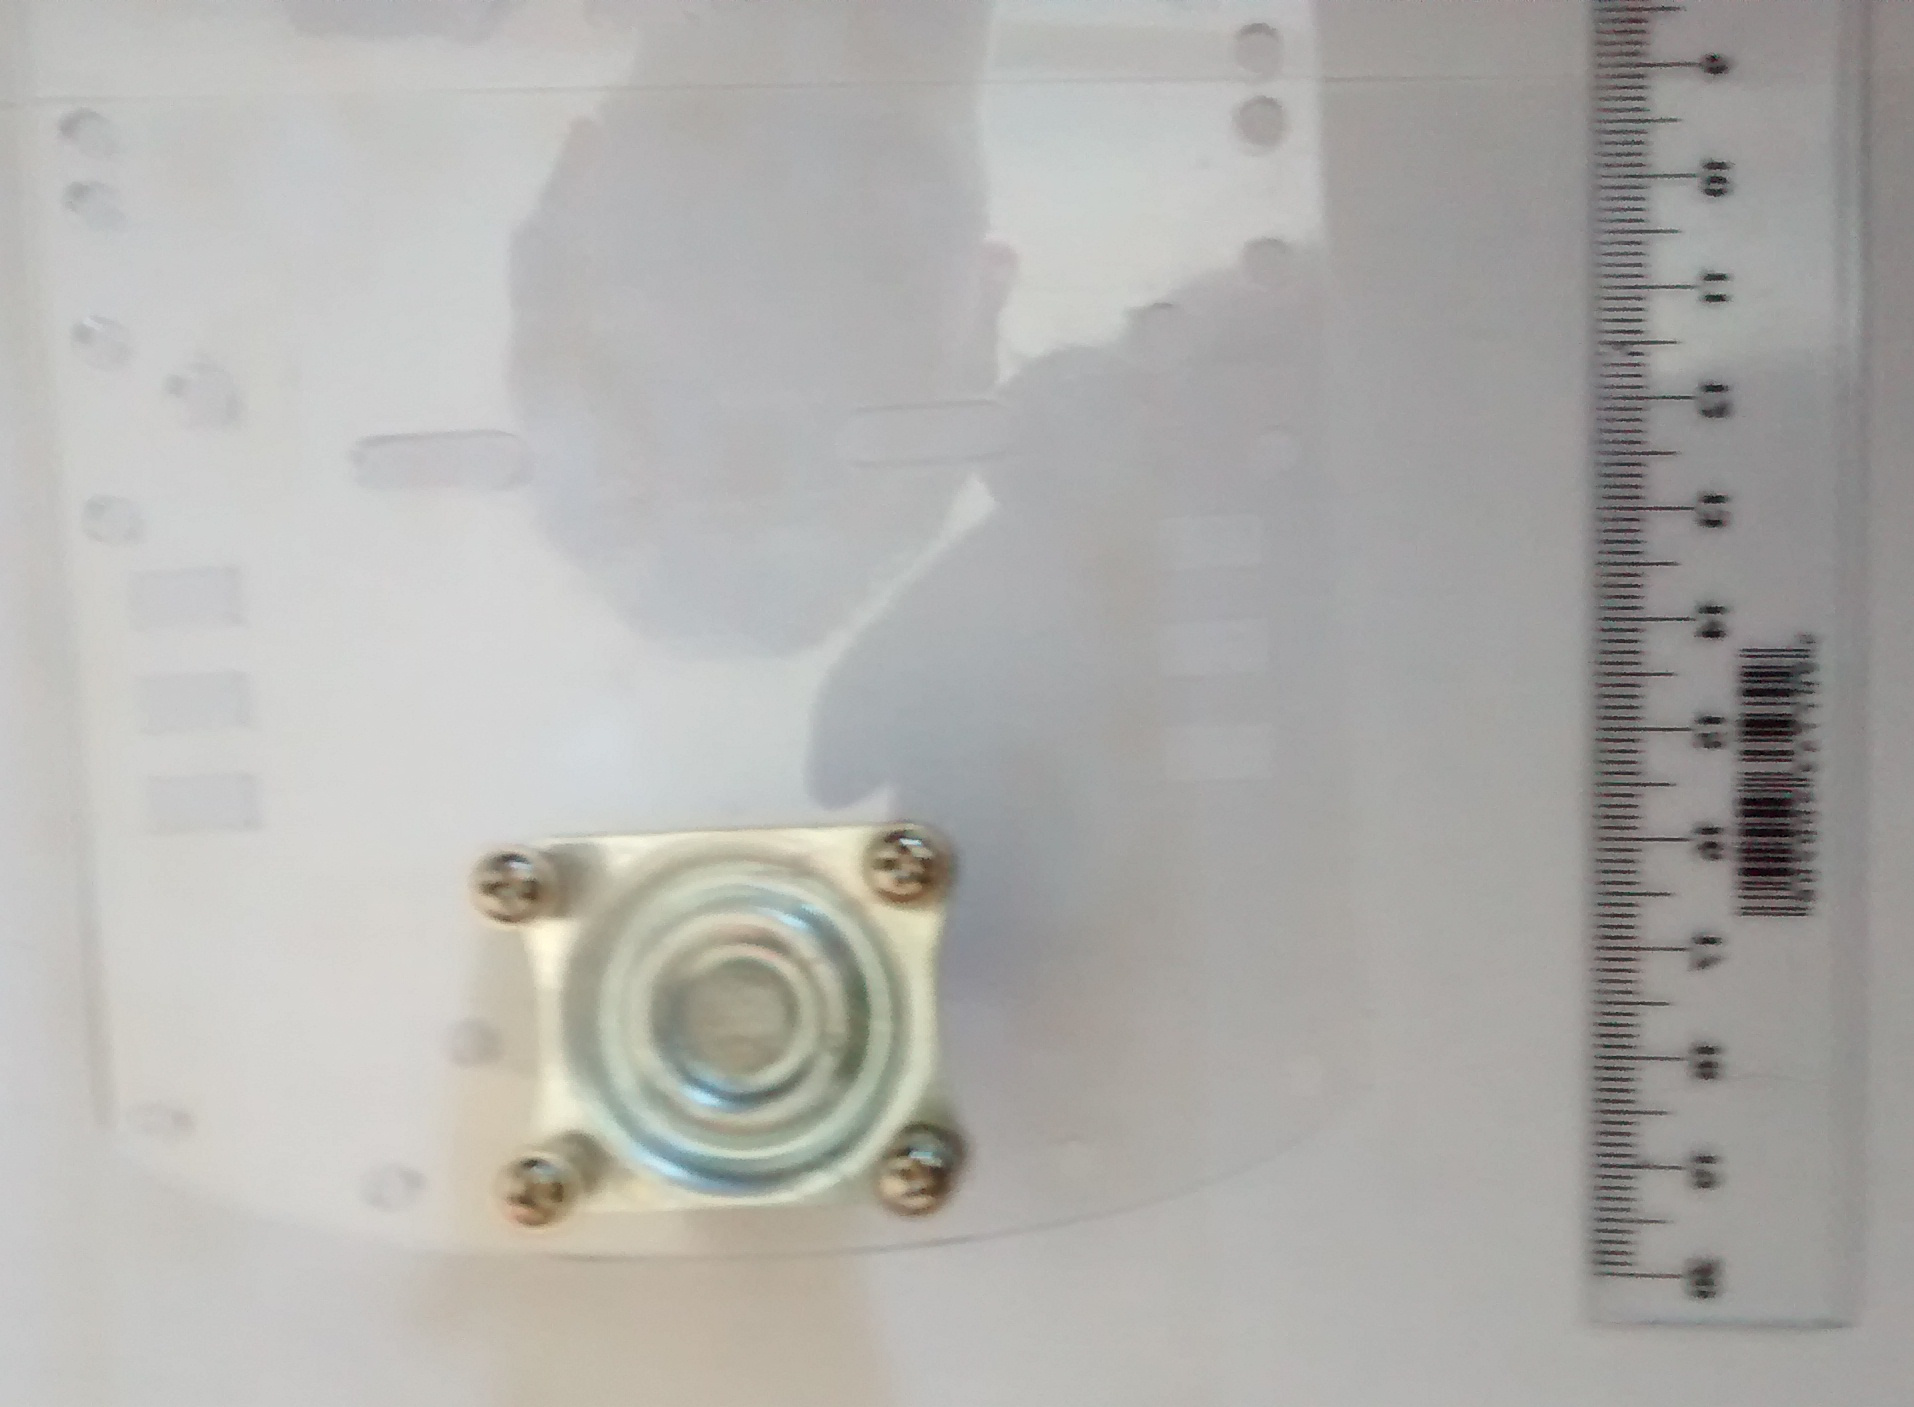
\includegraphics[width=\SCALE
	\paperwidth]{podstawa-3}
	\caption{podstawa}
\end{figure}

\begin{figure}[H]
	\centering
	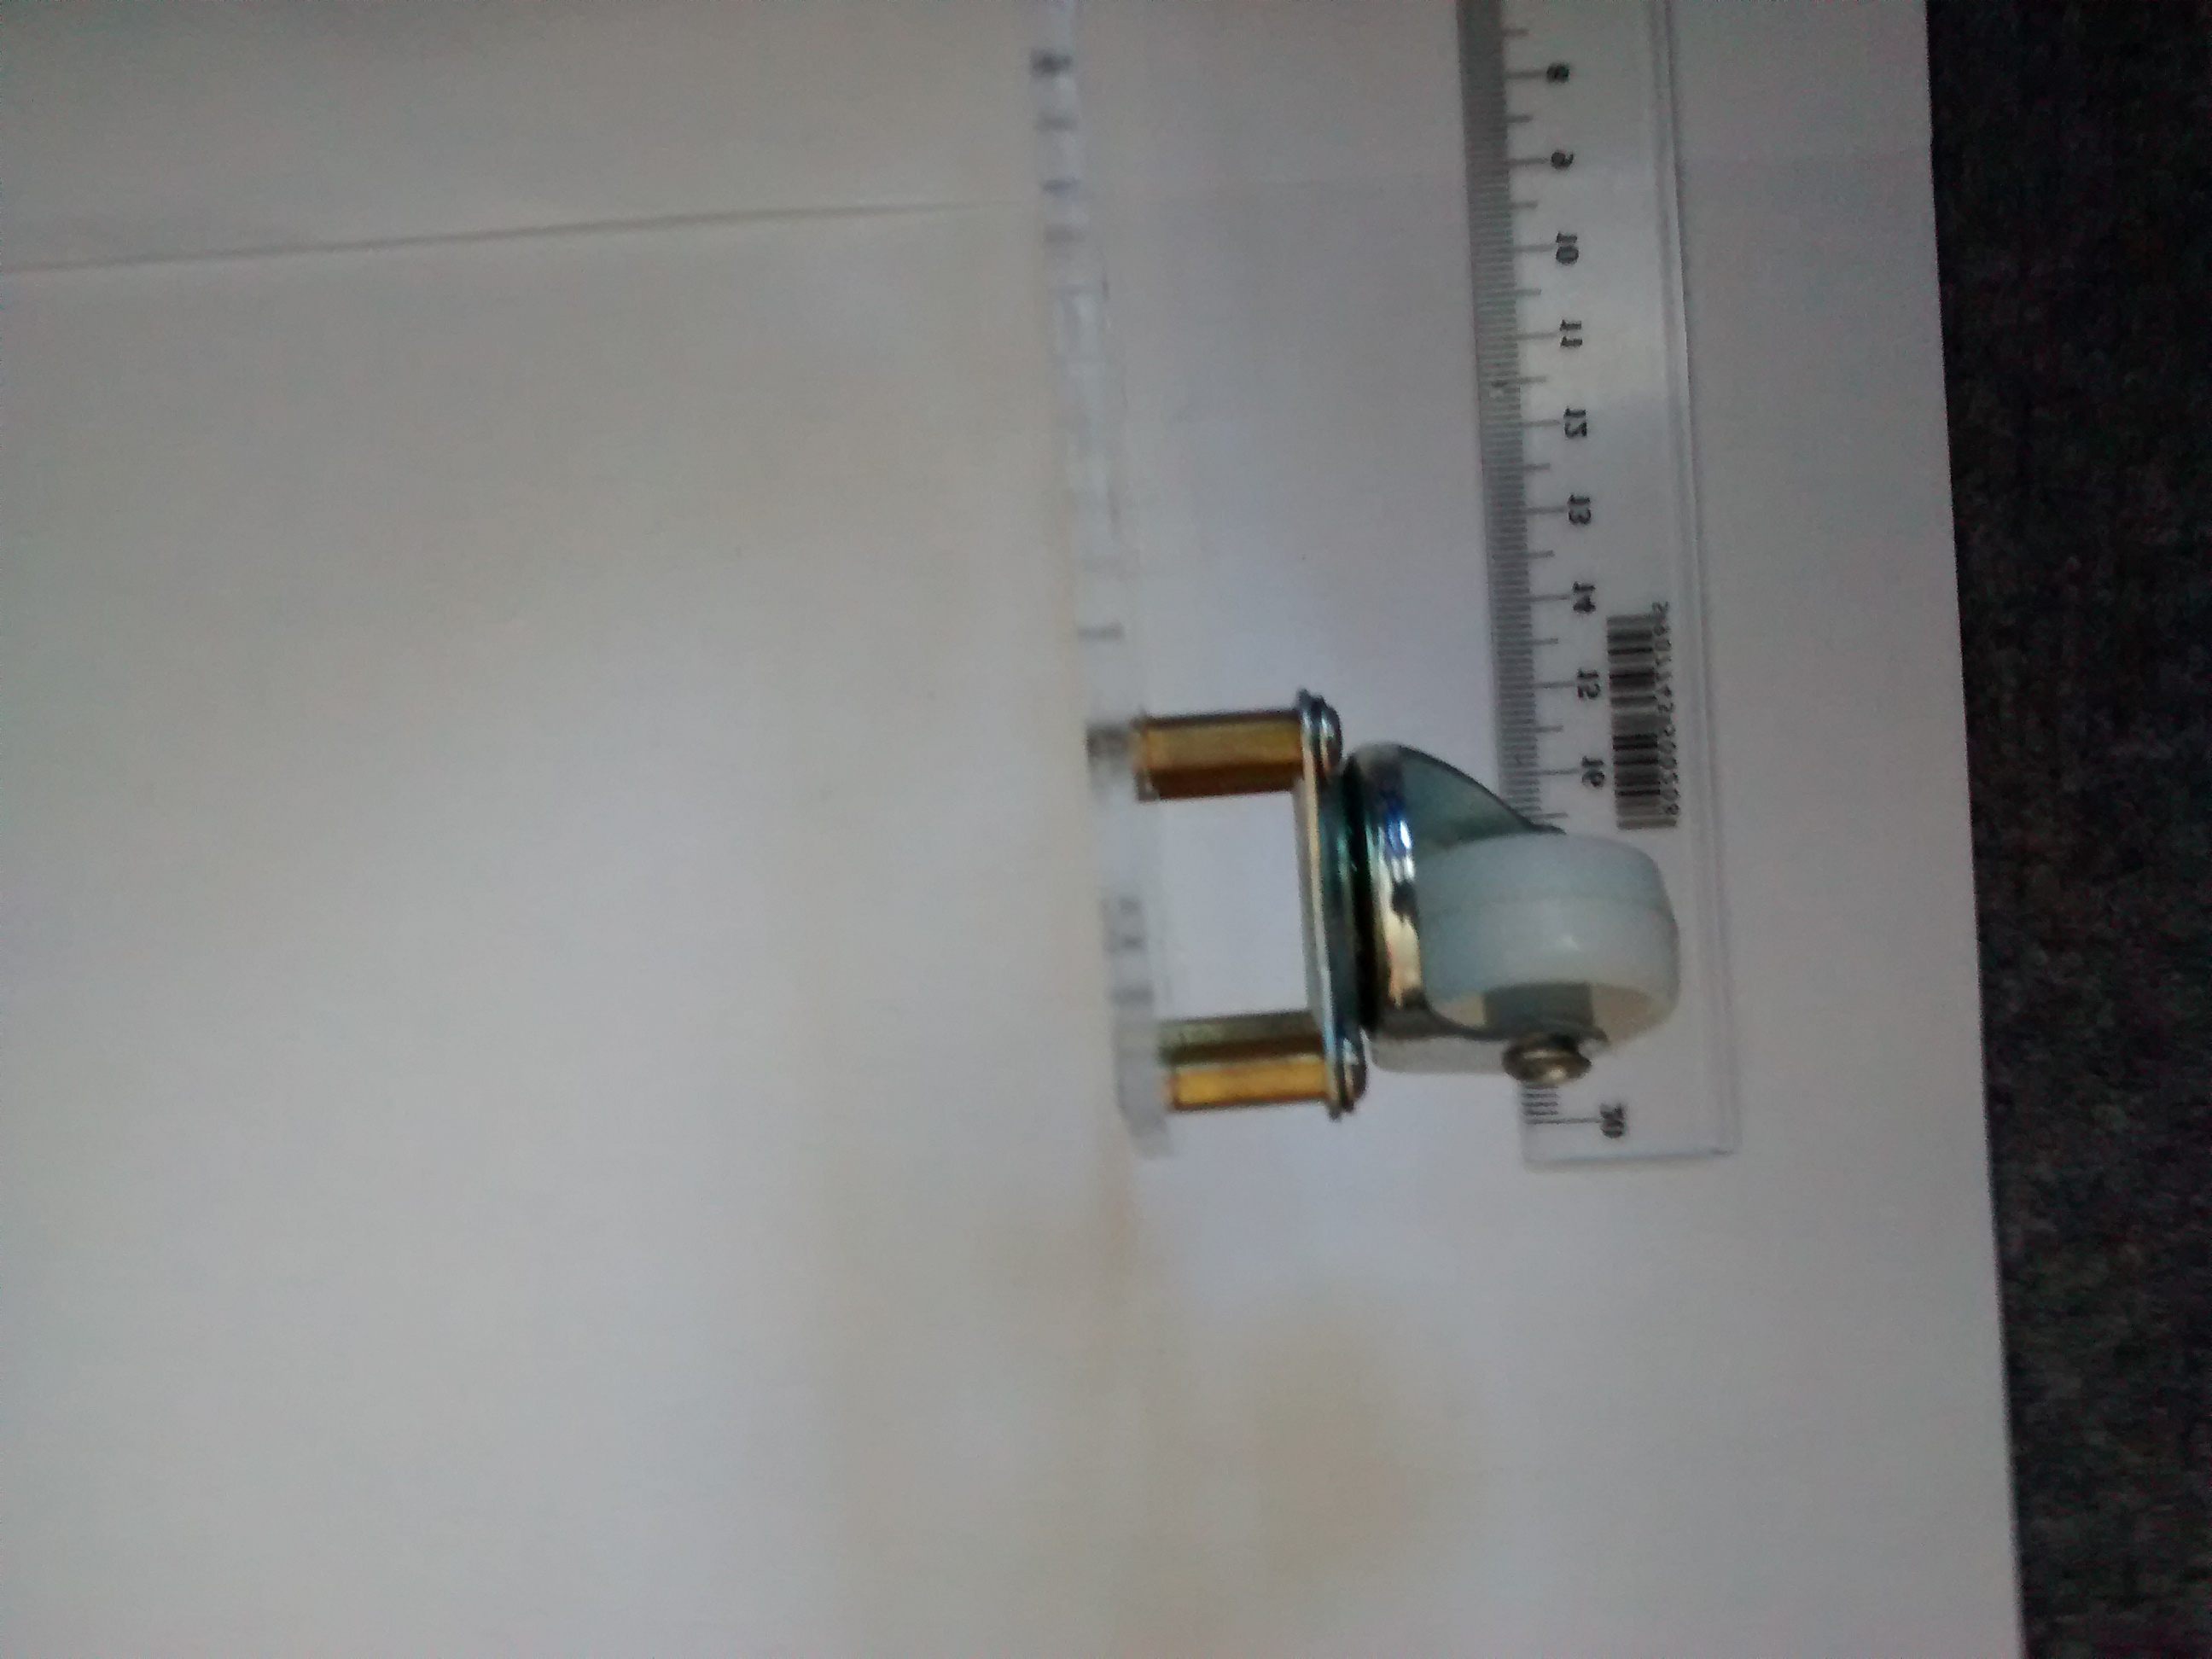
\includegraphics[width=\SCALE
	\paperwidth]{podstawa-4}
	\caption{podstawa}
\end{figure}

\begin{figure}[H]
	\subsubsection{czujnik}
	Czujnik wyposażony jest w diodę LED, którą podświetla trasę. Unika tym poleganiu na zewnętrznych źródłach światła. Następnie mierzy wartość światła odbitego. Działa w podczerwieni. Czujnik wyposażony jest w przerzutnik schmitta, który niestety bardziej przeszkadza niż pomaga. Lepiej jest wykorzystać czujniki w pełni analogowe. Czujnik ma również diodę diagnostyczną, która świeci w świetle widzialnym aby ułatwić diagnozowanie.
	
	\centering
	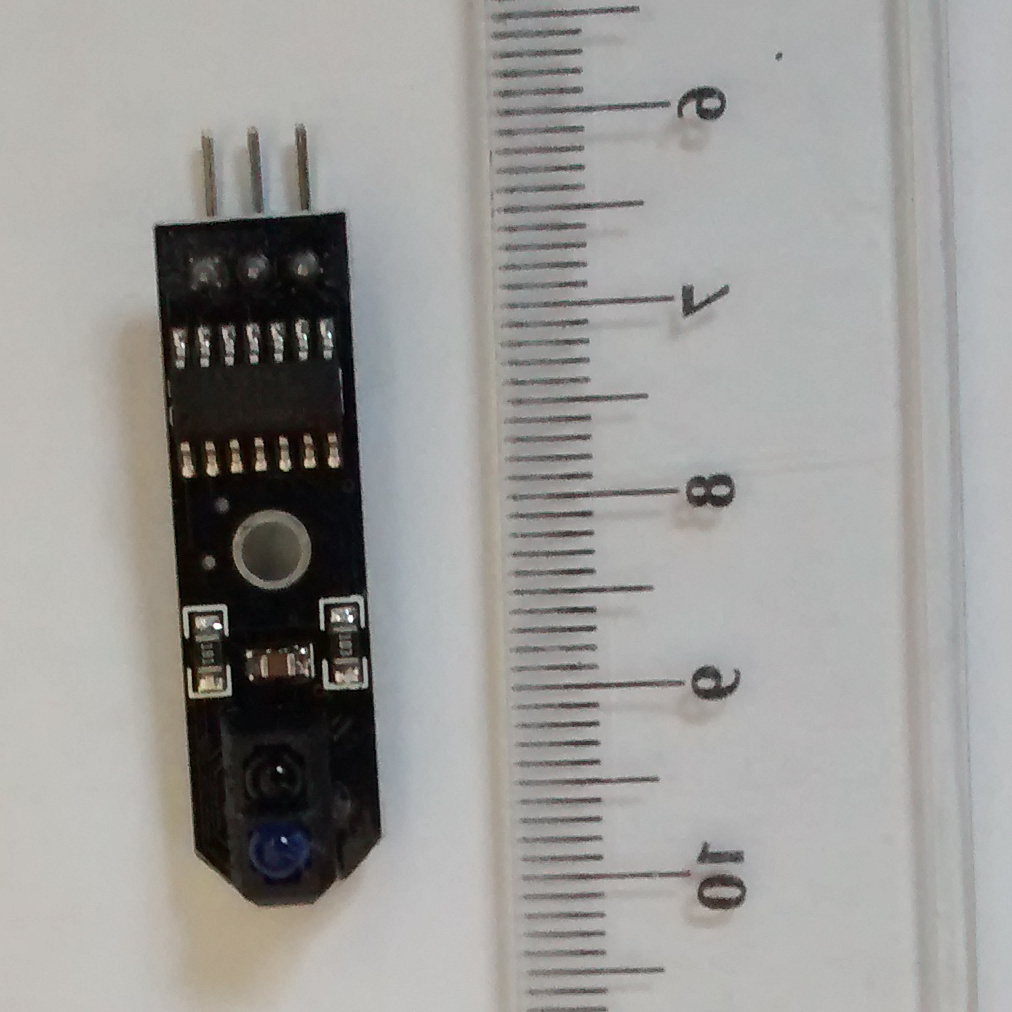
\includegraphics[width=\SCALE
	\paperwidth]{czujnik}
	\caption{czujnik}

\end{figure}

\begin{figure}[H]
	\subsubsection{Mocowanie czujnika}
	Czujnik zamocowany jest na pociętym pręcie i przykręcony do podwozia. Odległość czujników należy dobrać eksperymentalnie w zależności od podłoża.	
	
	\centering
	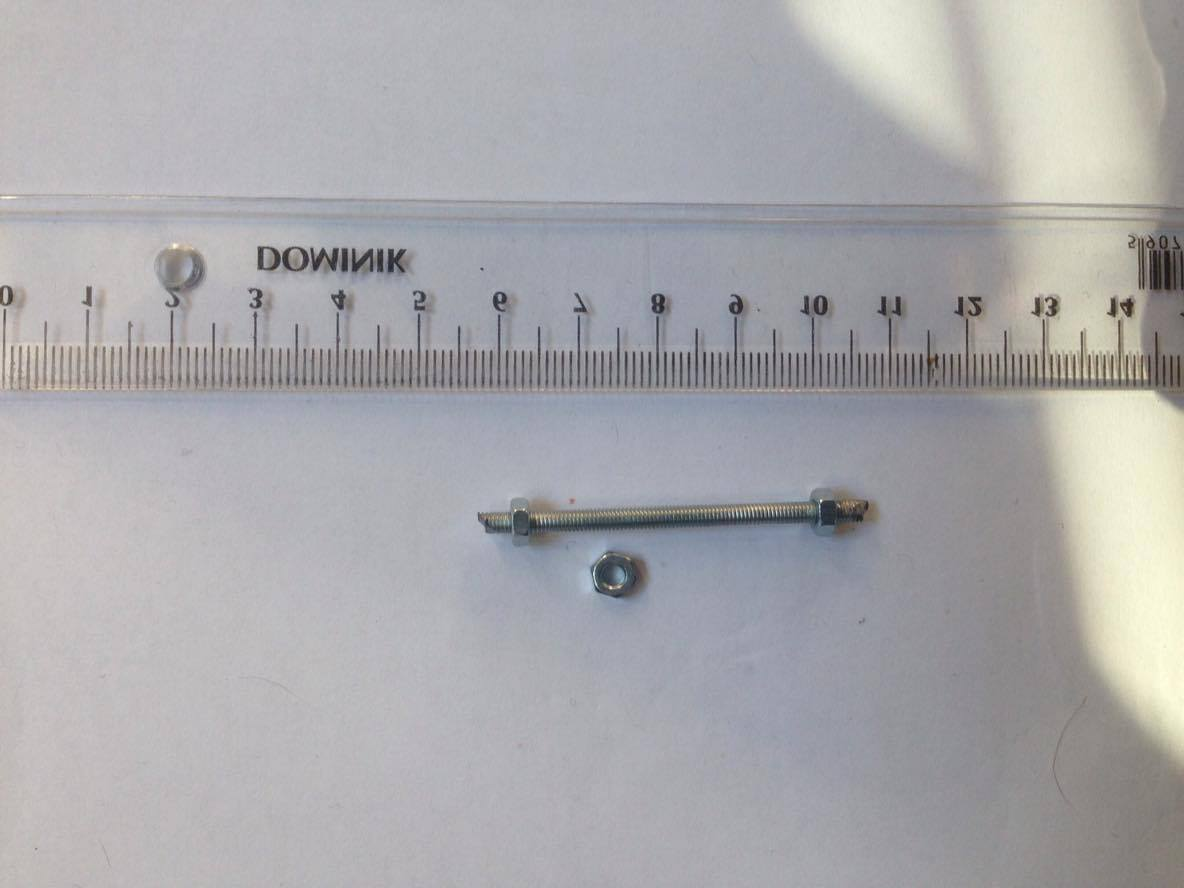
\includegraphics[width=\SCALE
	\paperwidth]{mocowanieCzujnika}
	\caption{Mocowanie czujnika}

\end{figure}


\begin{figure}[H]
	\subsubsection{pojemnik na baterie}
	Łączy 6 baterii szeregowo w wyniku czego napięcie wyjściowe wynosi około 9V.


	\centering
	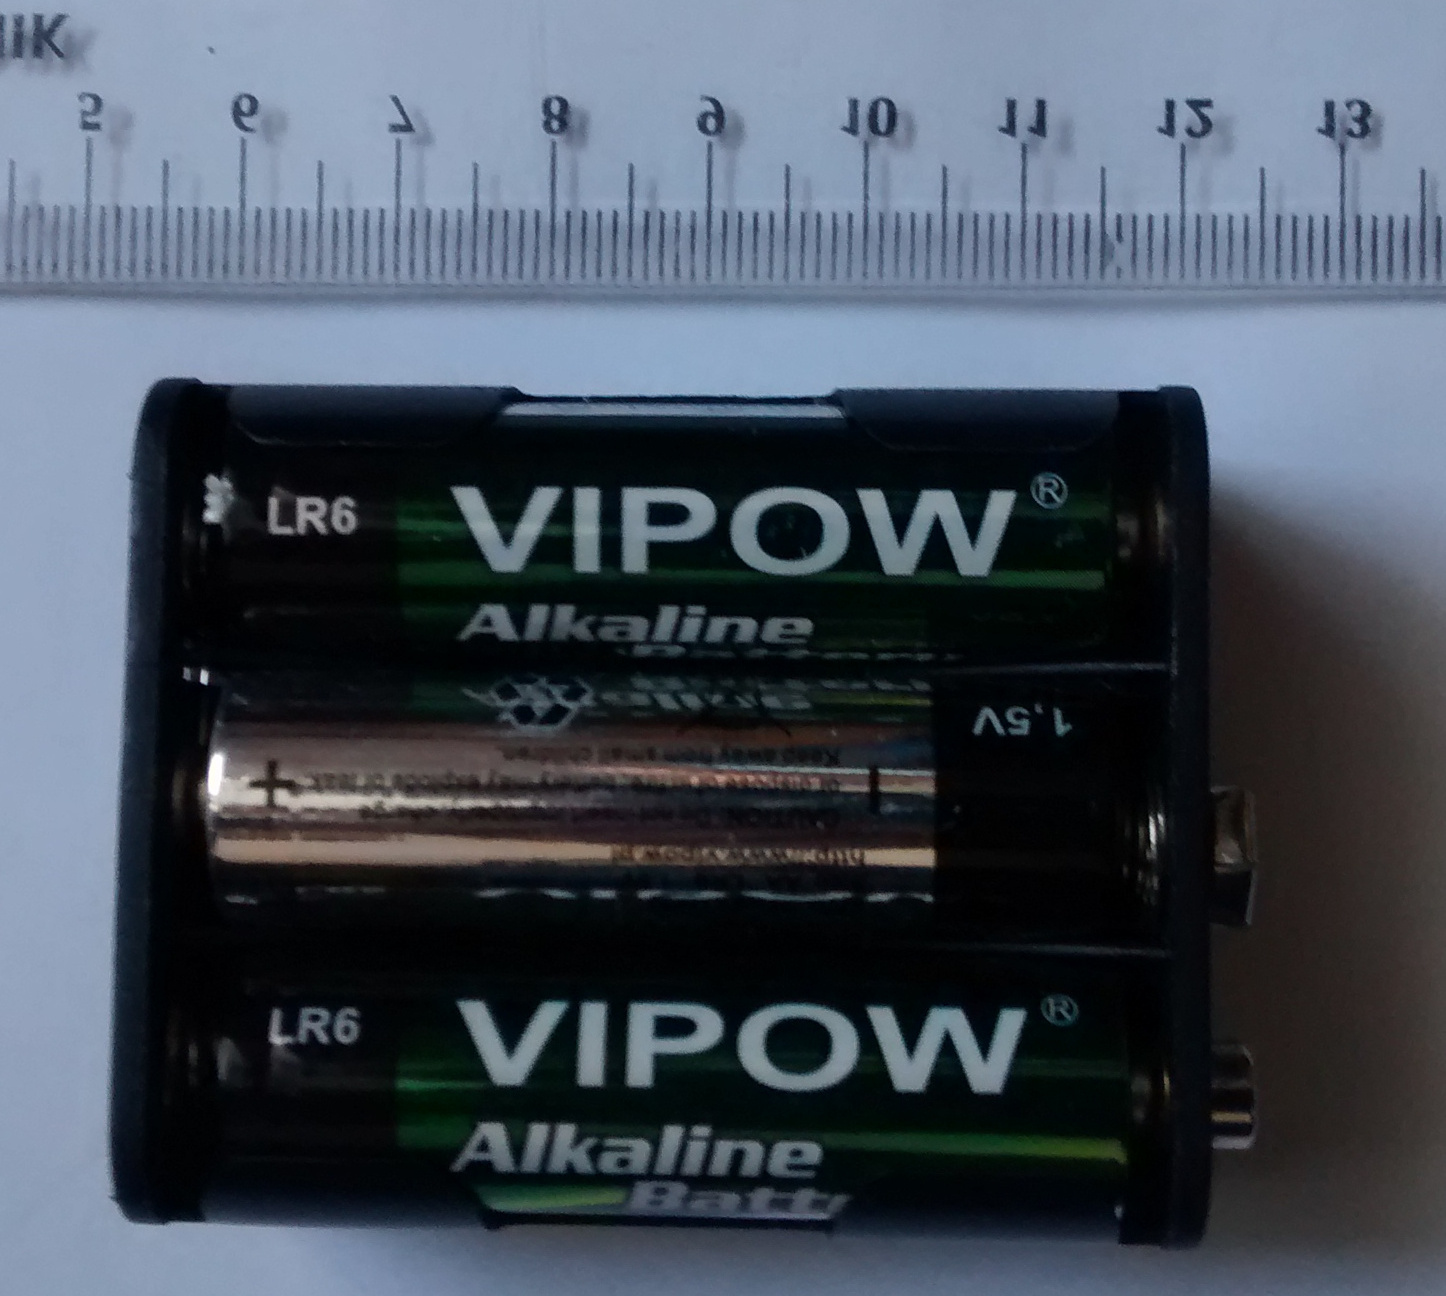
\includegraphics[width=\SCALE
	\paperwidth]{pojemnik-1}
	\caption{pojemnik bok}
	

	
\end{figure}
	\begin{figure}[H]
		\centering
		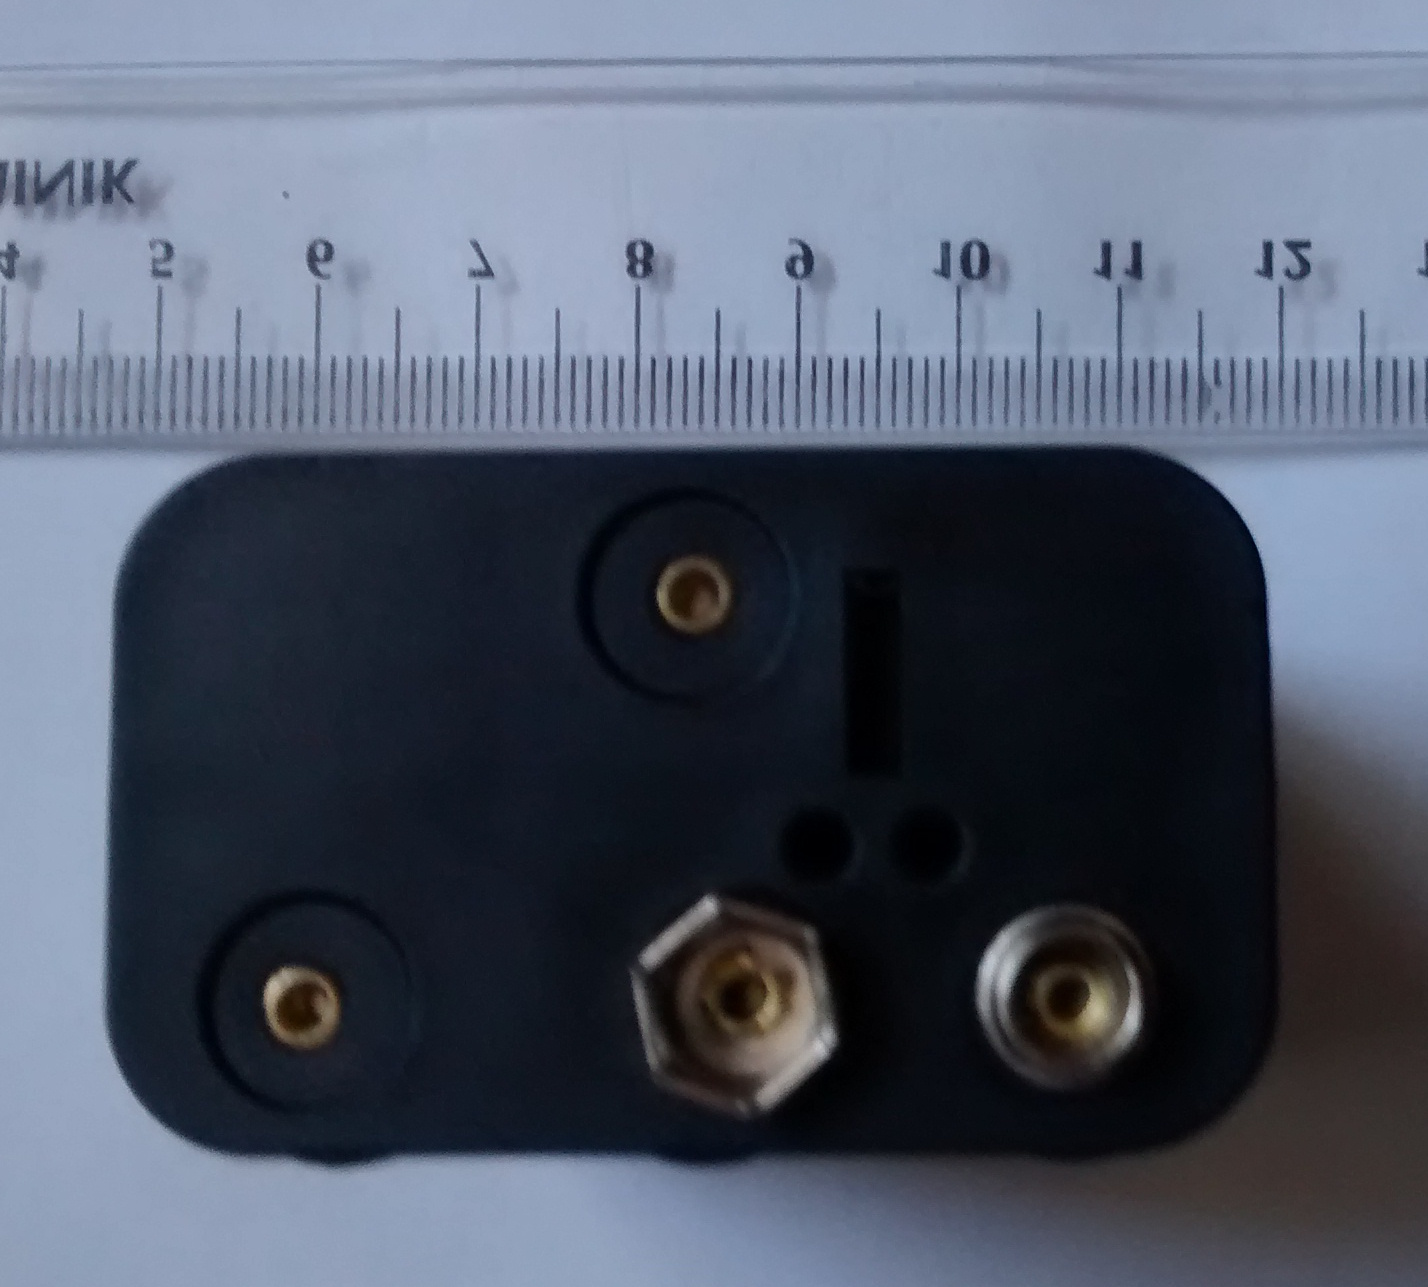
\includegraphics[width=\SCALE
		\paperwidth]{pojemnik-2}
		\caption{pojemnik góra}
	\end{figure}	


\subsubsection{wtyczka}
\begin{figure}[H]
	\centering
	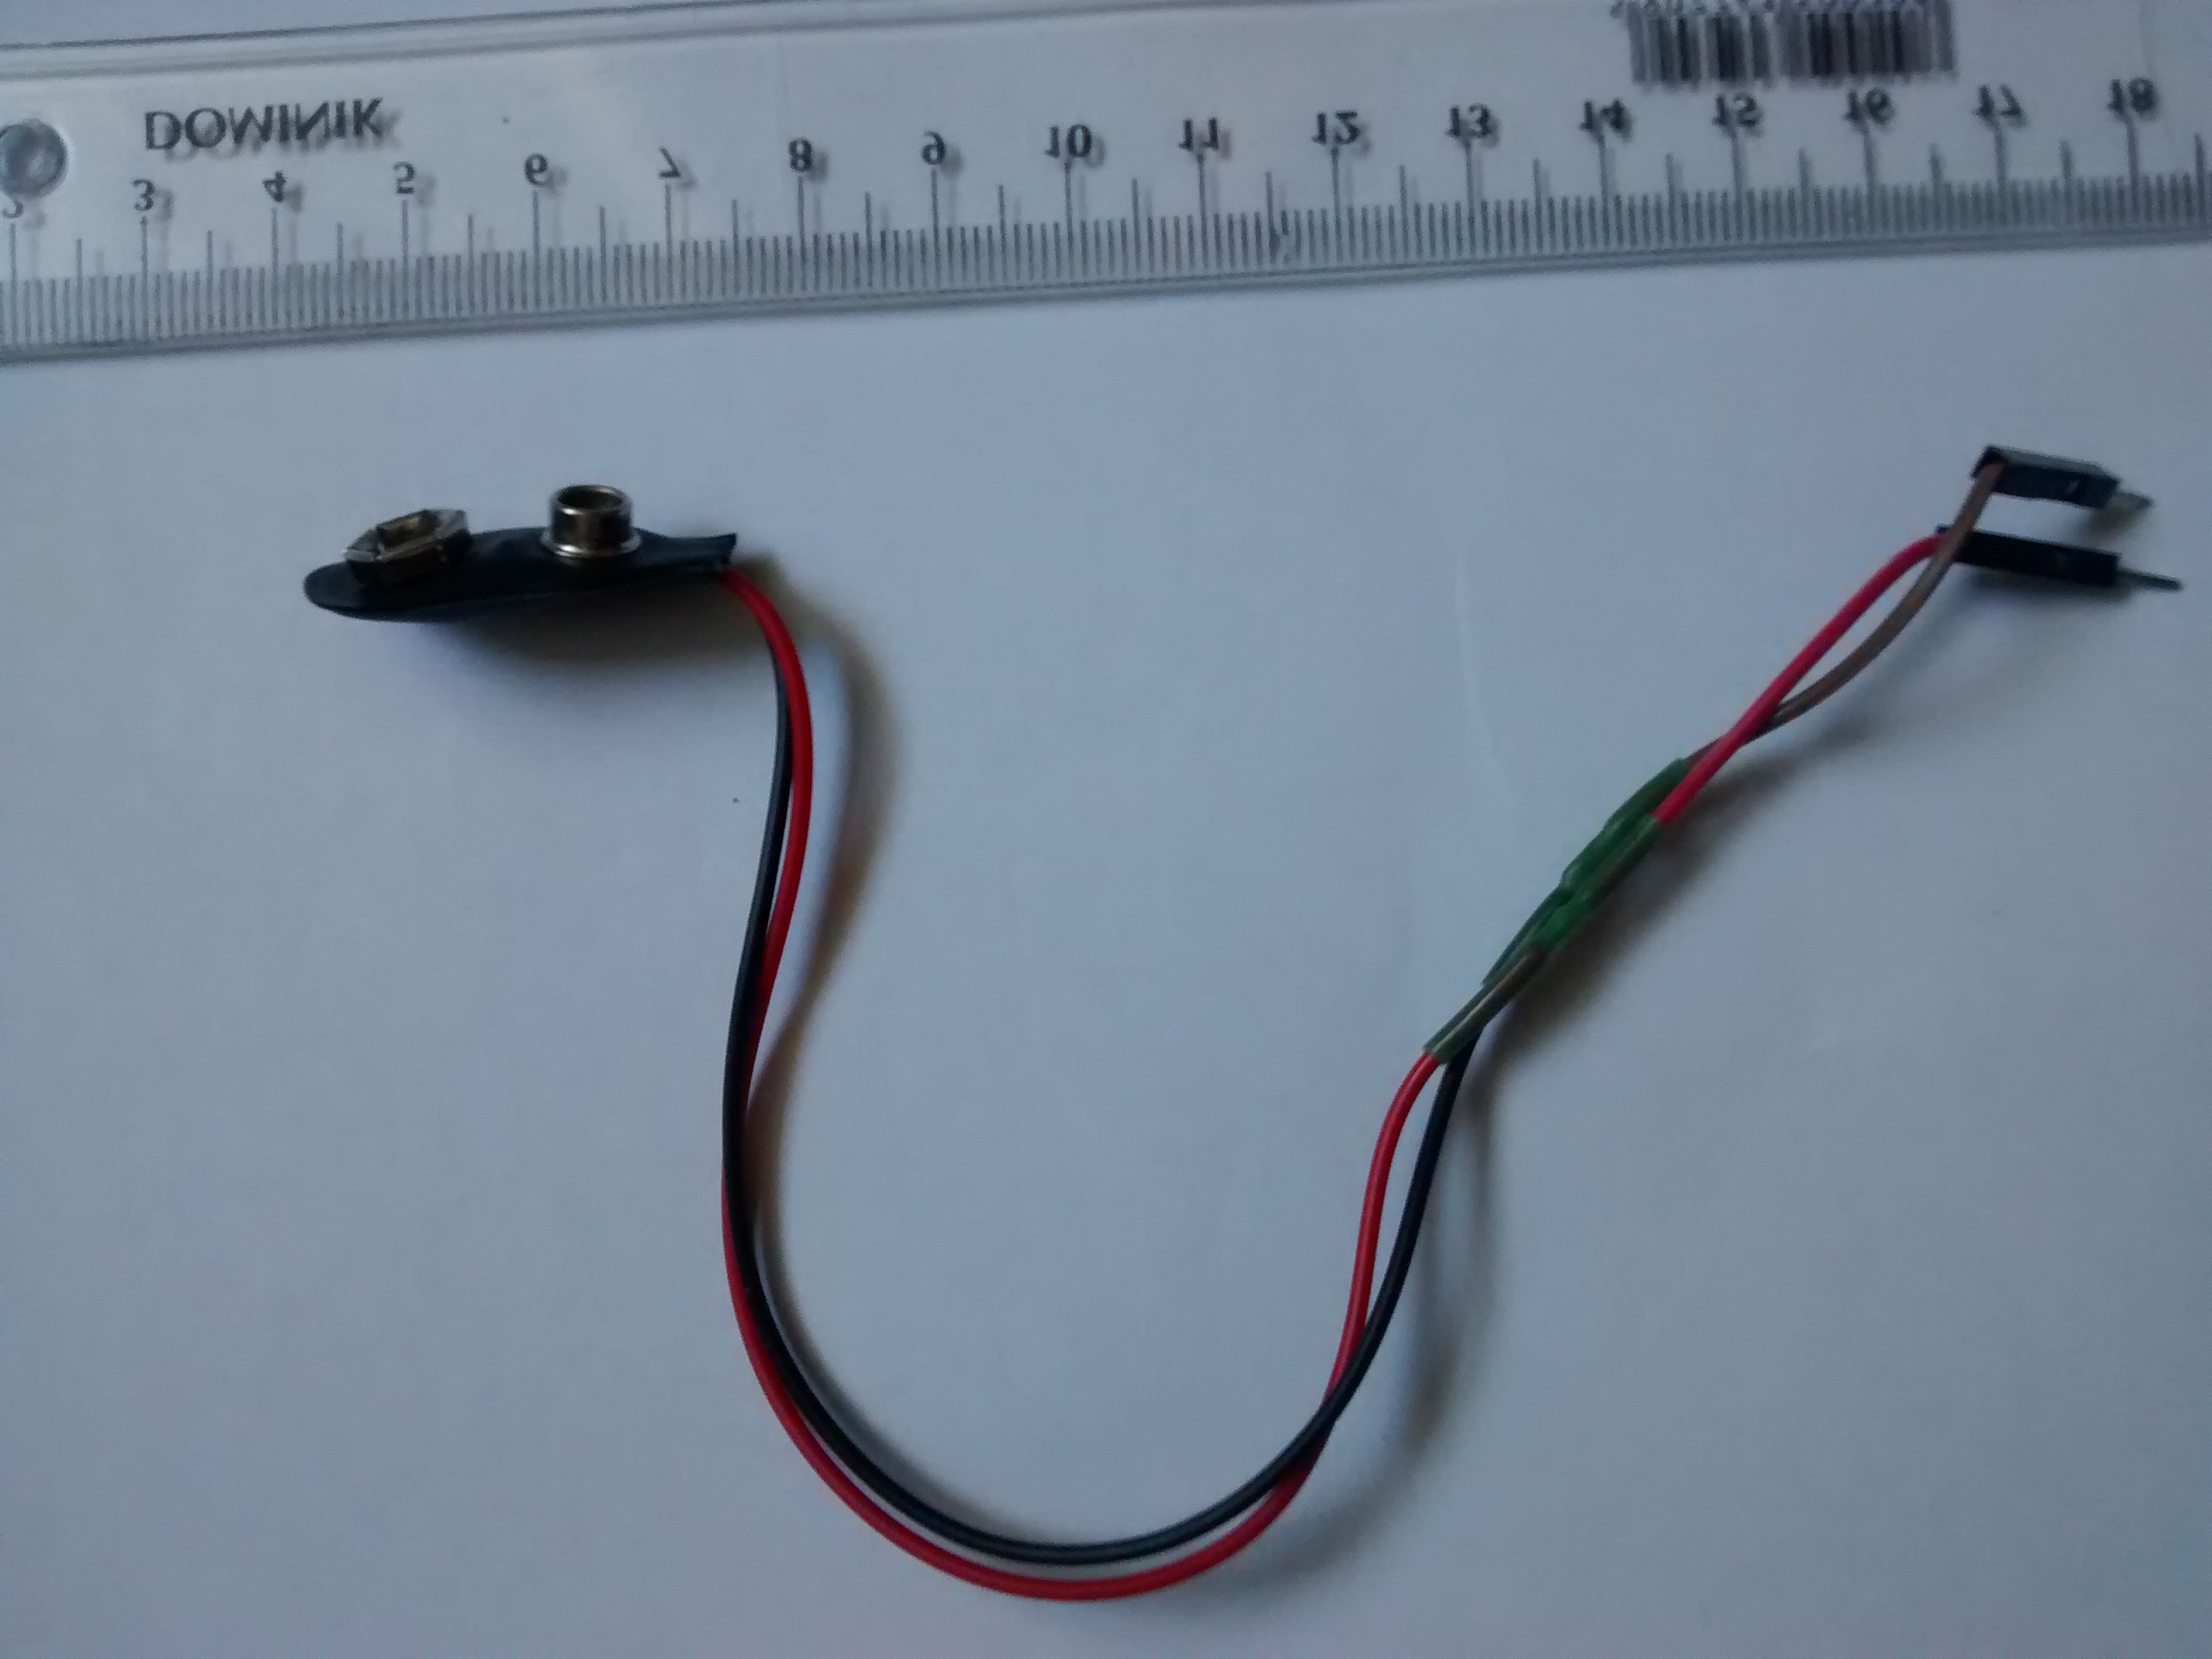
\includegraphics[width=\SCALE
	\paperwidth]{zlaczka}
	\caption{wtyczka}
\end{figure}


\begin{figure}[H]

	\subsubsection{płytka pcb}
Używana do wyprowadzenia wyjść Atmegi oraz jako miejsce na stabilizator 5V kondensatory filtrujące,	oraz rezystor i przycisk do resetu. Łączy elementy. Wymiary 7x9cm.

	\centering
	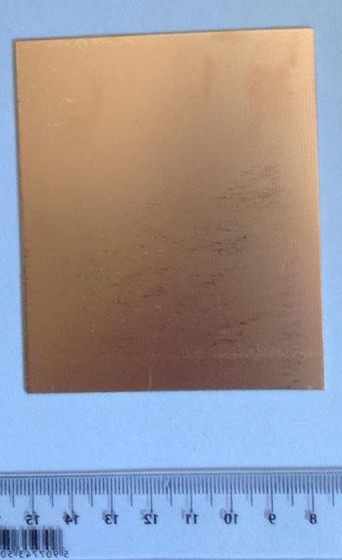
\includegraphics[width=\SCALE
	\paperwidth]{plytka}
	\caption{Płytka PCB}
\end{figure}
\subsubsection{kondenstor}
	\paragraph{68nF}
Wykorzystywany jest do tłumienia zakłóceń powodowanych przez silnik. Można wykorzystać również kondesatory 100nF.
	\paragraph{100nF}
	Wykorzystywany jest do tłumienia zakłóceń w układzie zasilania. Jeden wykorzystany do resetu Atmegi.
	\paragraph{22pF}
	Wymagany przez oscylator.
\subsubsection{przycisk monostabliny}
	Ręcznie aktywuje reset Atmegi.
\subsubsection{stabilizator 7805}
	Dostarcza stabilne 5V dla zasilania czujników oraz Atmegi, .
	
\section{Płytka}
\subsection{Projekt}
\subsection{Termotransfer}
\subsubsection{Przygotowania}
Projekt należy wydrukować na papierze kredowym drukarką laserową. Uwaga na zachowanie skali wydruku. Następnie można przejść do przygotowanie miedzianej płytki. Należy oczyścić powierzchnie z tlenków wodnym papierem ściernym 1000. Kolejnie wyczyścić z zabrudzeń mocnym alkoholem. Tak przygotowana płytka jest gotowa na termotransfer.
\subsubsection{Termotransfer}
Do termotransferu potrzebne jest żelazko. Należy je rozgrzać na dwie kropki ok (150$^\circ$C).

Dobrze jest też przygotować odpowiednie stanowisko, by nie przesunąć płytki względem druku podczas operacji.

Można zastosować metodę gdzie żelazko jest na górze lub na dole względem płytki. W wielu poradnikach można znaleźć różne informacje na ten temat, jednak nie wiemy jaka metoda, temperatura, czas jest najlepszy. Za duża temperatura zżłóci papier, za niska uniemożliwi termotransfer.

My zastosowaliśmy metodę górną z podkładem z zeszytu i ręczników papierowych. Nie prasowaliśmy też bezpośrednio po papierze kredowym, tylko przykryliśmy go papierem do pieczenia. W ramach nakładki na papier kredowy powinna też sprawdzić się bawełniana szmatka.

Papier kredowy drukiem do dołu przylegał do miedzianej płytki. Temperatura podgrzewała toner umożliwiając przeniesienie warstwy tonera na miedź. By zwiększyć docisk co 40 sek. prasowaliśmy płytkę 40 sek. papierową kulką, umożliwiło to dokładniejszy i silniejszy docisk niż żelazkiem. Wykonaliśmy sześć takich zmian.

Toner nie powinien łatwo schodzić z płytki, jeśli schodzi po przeciągnięciu palcem, operacje lepiej powtórzyć, stosując trochę wyższą temperaturę lub wydłużając czas grzania.
\begin{figure}[H]
	\centering
	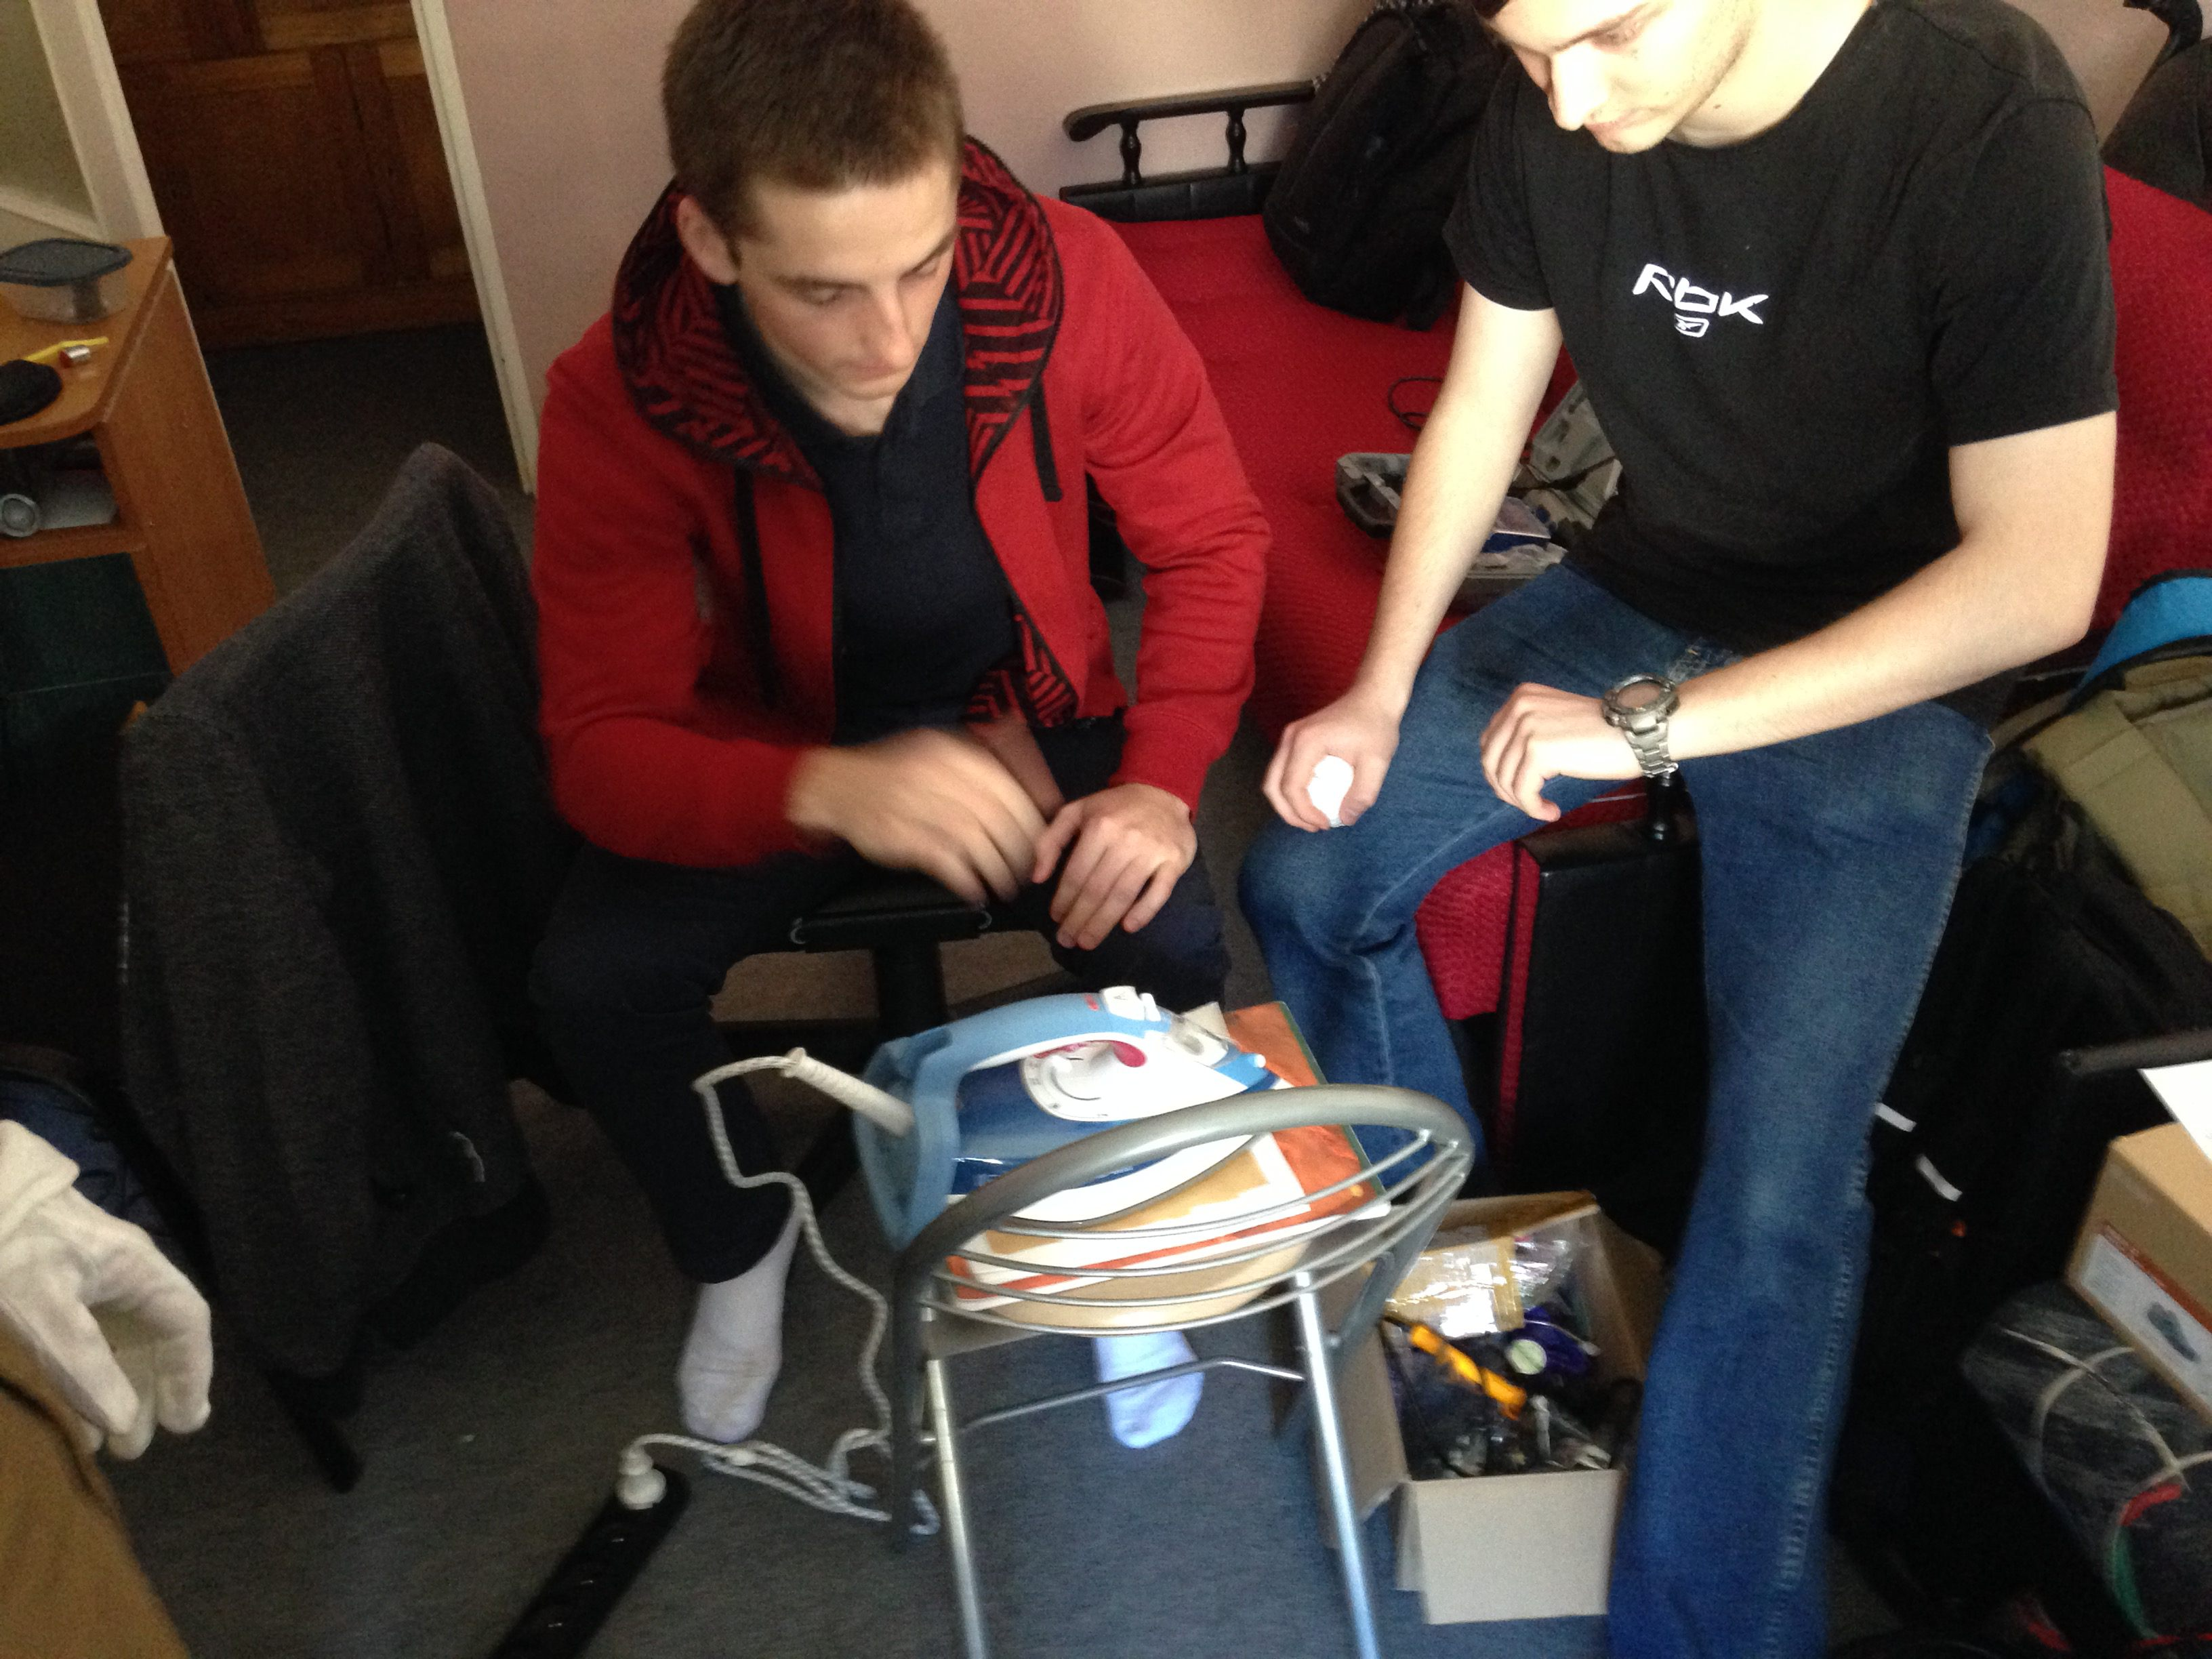
\includegraphics[width=\SCALE
	\paperwidth]{termotransfer-1}
	\caption{termotransfer - nagrzewanie żelazkiem}
\end{figure}

\subsubsection{Poprawki}

\begin{figure}[H]
Następnie trzeba usunąć papier kredowy. Można to zrobić w ciepłej wodzie z płynem do mycia naczyń, należy poczekać, aż nasiąknie. Kolejnie delikatnie go usuwamy. W niektórych miejscach nie pokrytych tonerem można znaleźć kredę. Jest to wysoce niepożądane, gdyż kreda utrudni dostęp roztworu do trawienia. Można ją usunąć np. wykałaczką.

	\centering
	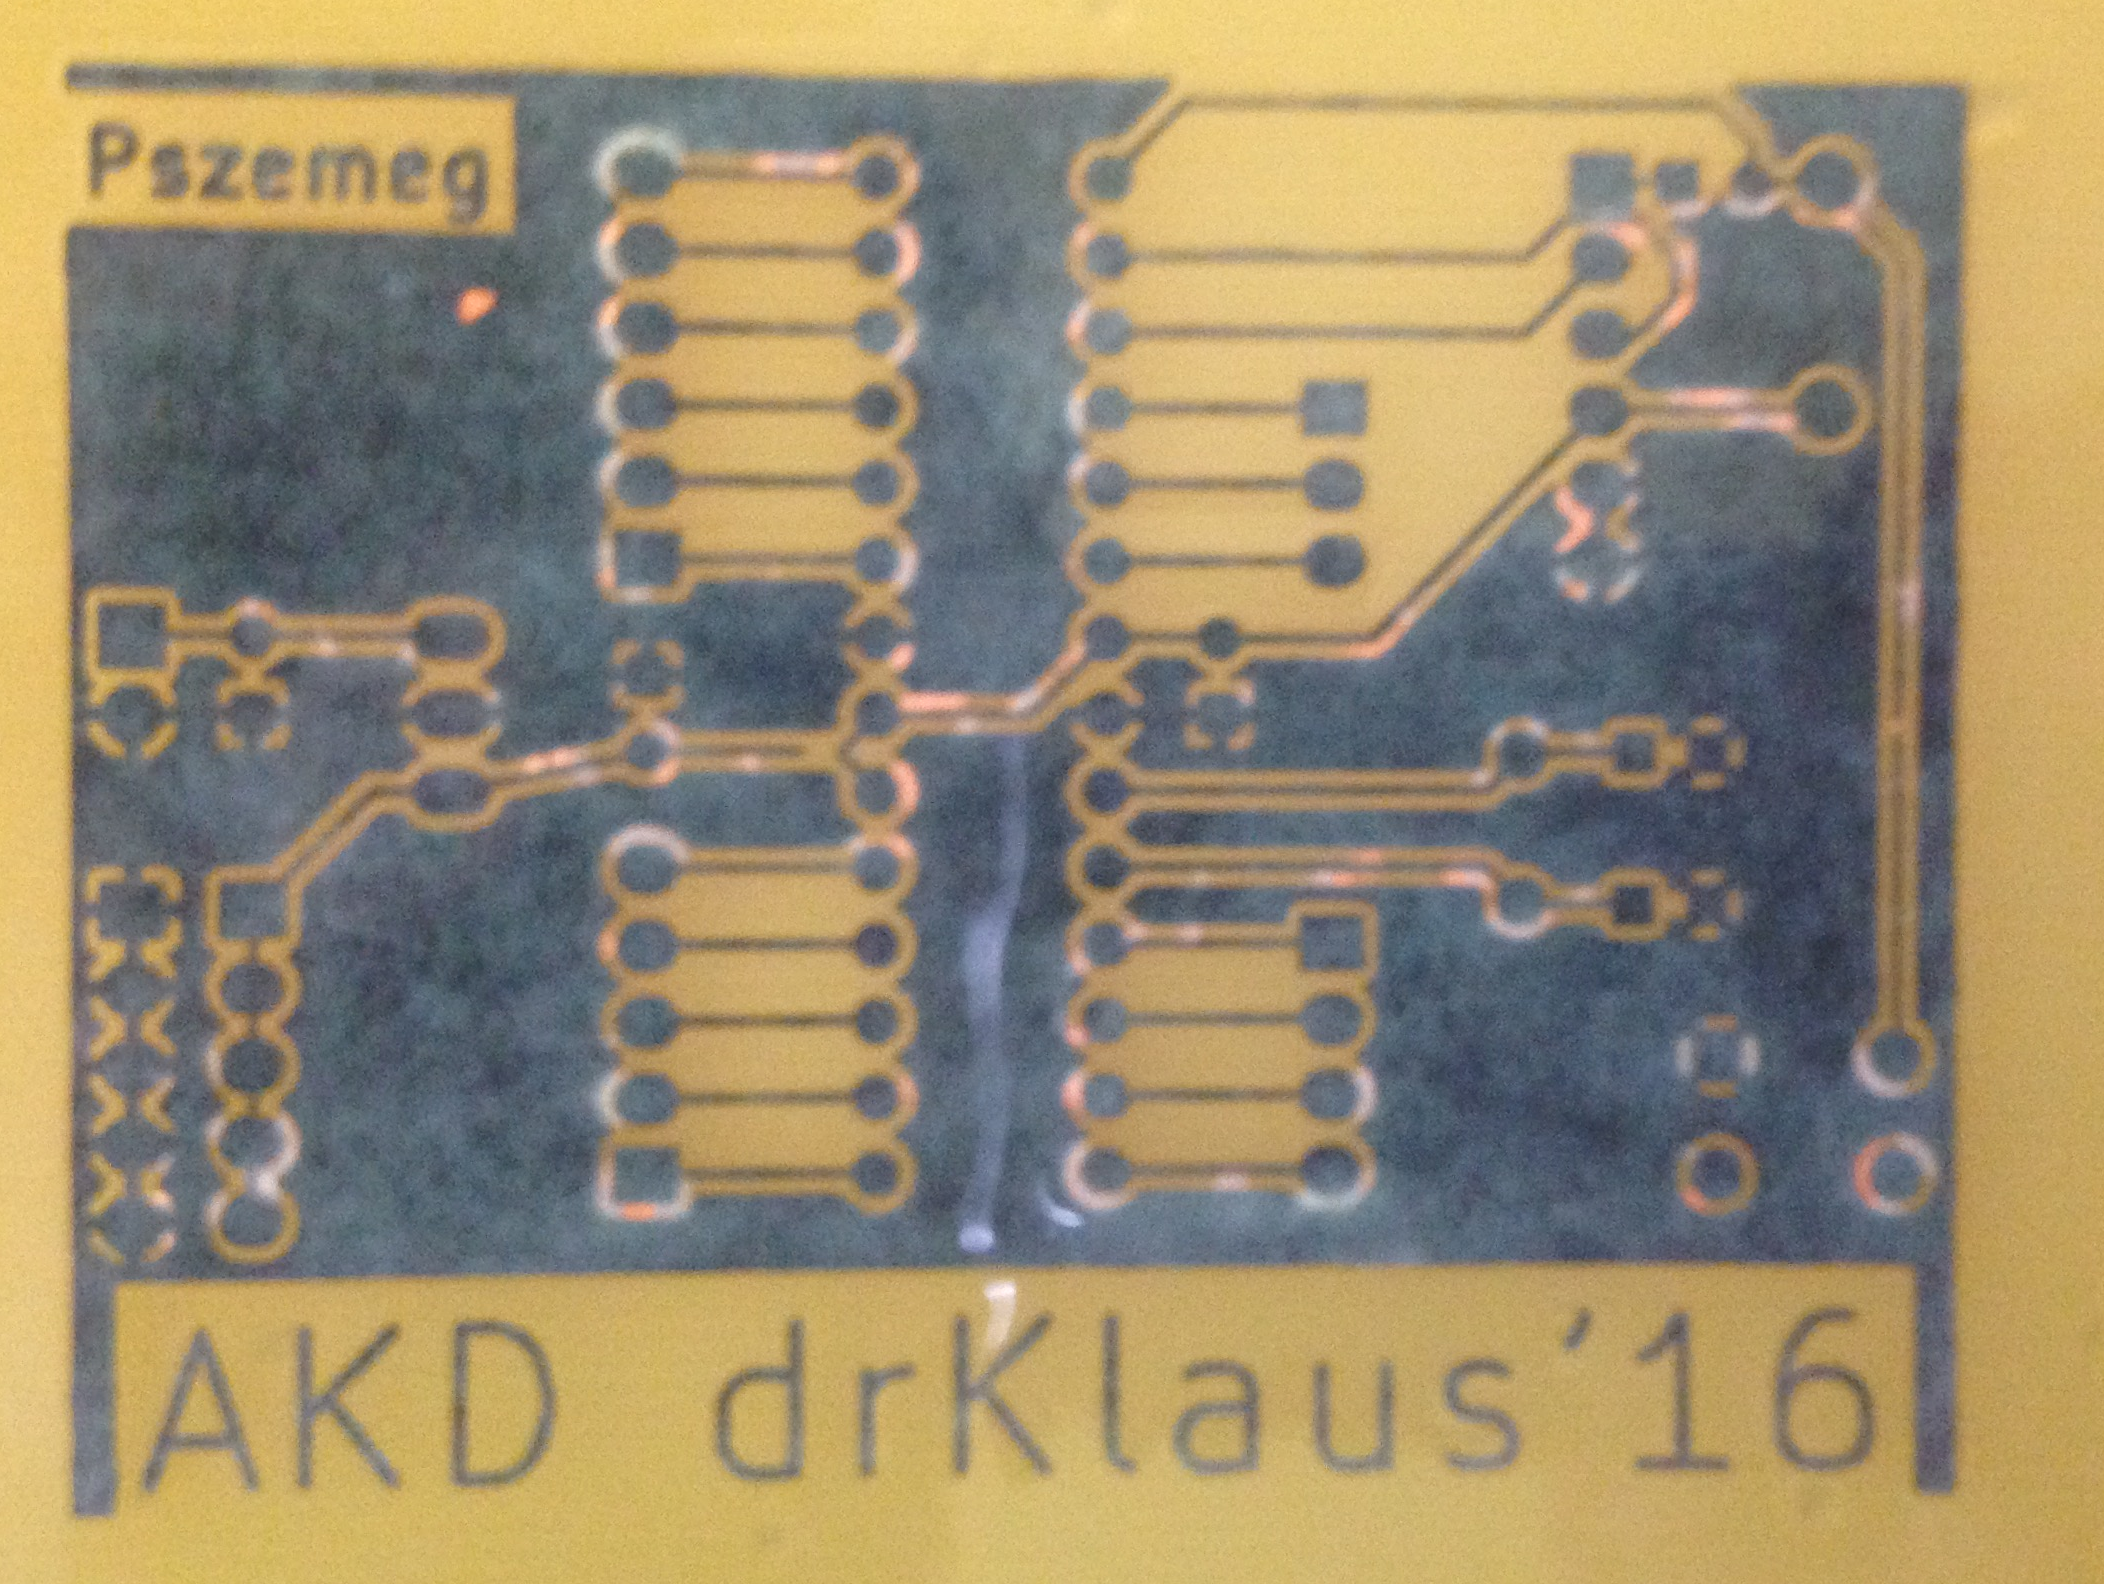
\includegraphics[width=\SCALE
	\paperwidth]{ZabrudzeniaKreda}
	\caption{Zabrudzenia kredą, tu niestety po wytrawianiu}
\end{figure}


Jeśli w niektórych miejscach ścieżki się nie przeniosły można je poprawić markerem niezmywalnym.
Jeśli termotransfer nie wyszedł po usunięciu tonera acetonem procedurę można rozpocząć od nowa.
\subsection{Wytrawanie}

Wytrawianie przeprowadziliśmy za pomocą roztworu nadsiarczanu sodowego b327. 0,1kg proszku należy rozpuścić w 0,5L wody. A następnie w temp. 40-50$^\circ$C przeprowadzić trawienie. Temperaturę można utrzymywać dolewając ciepłej wody do zewnętrznego pojemnika.

\begin{figure}[H]
	\centering
	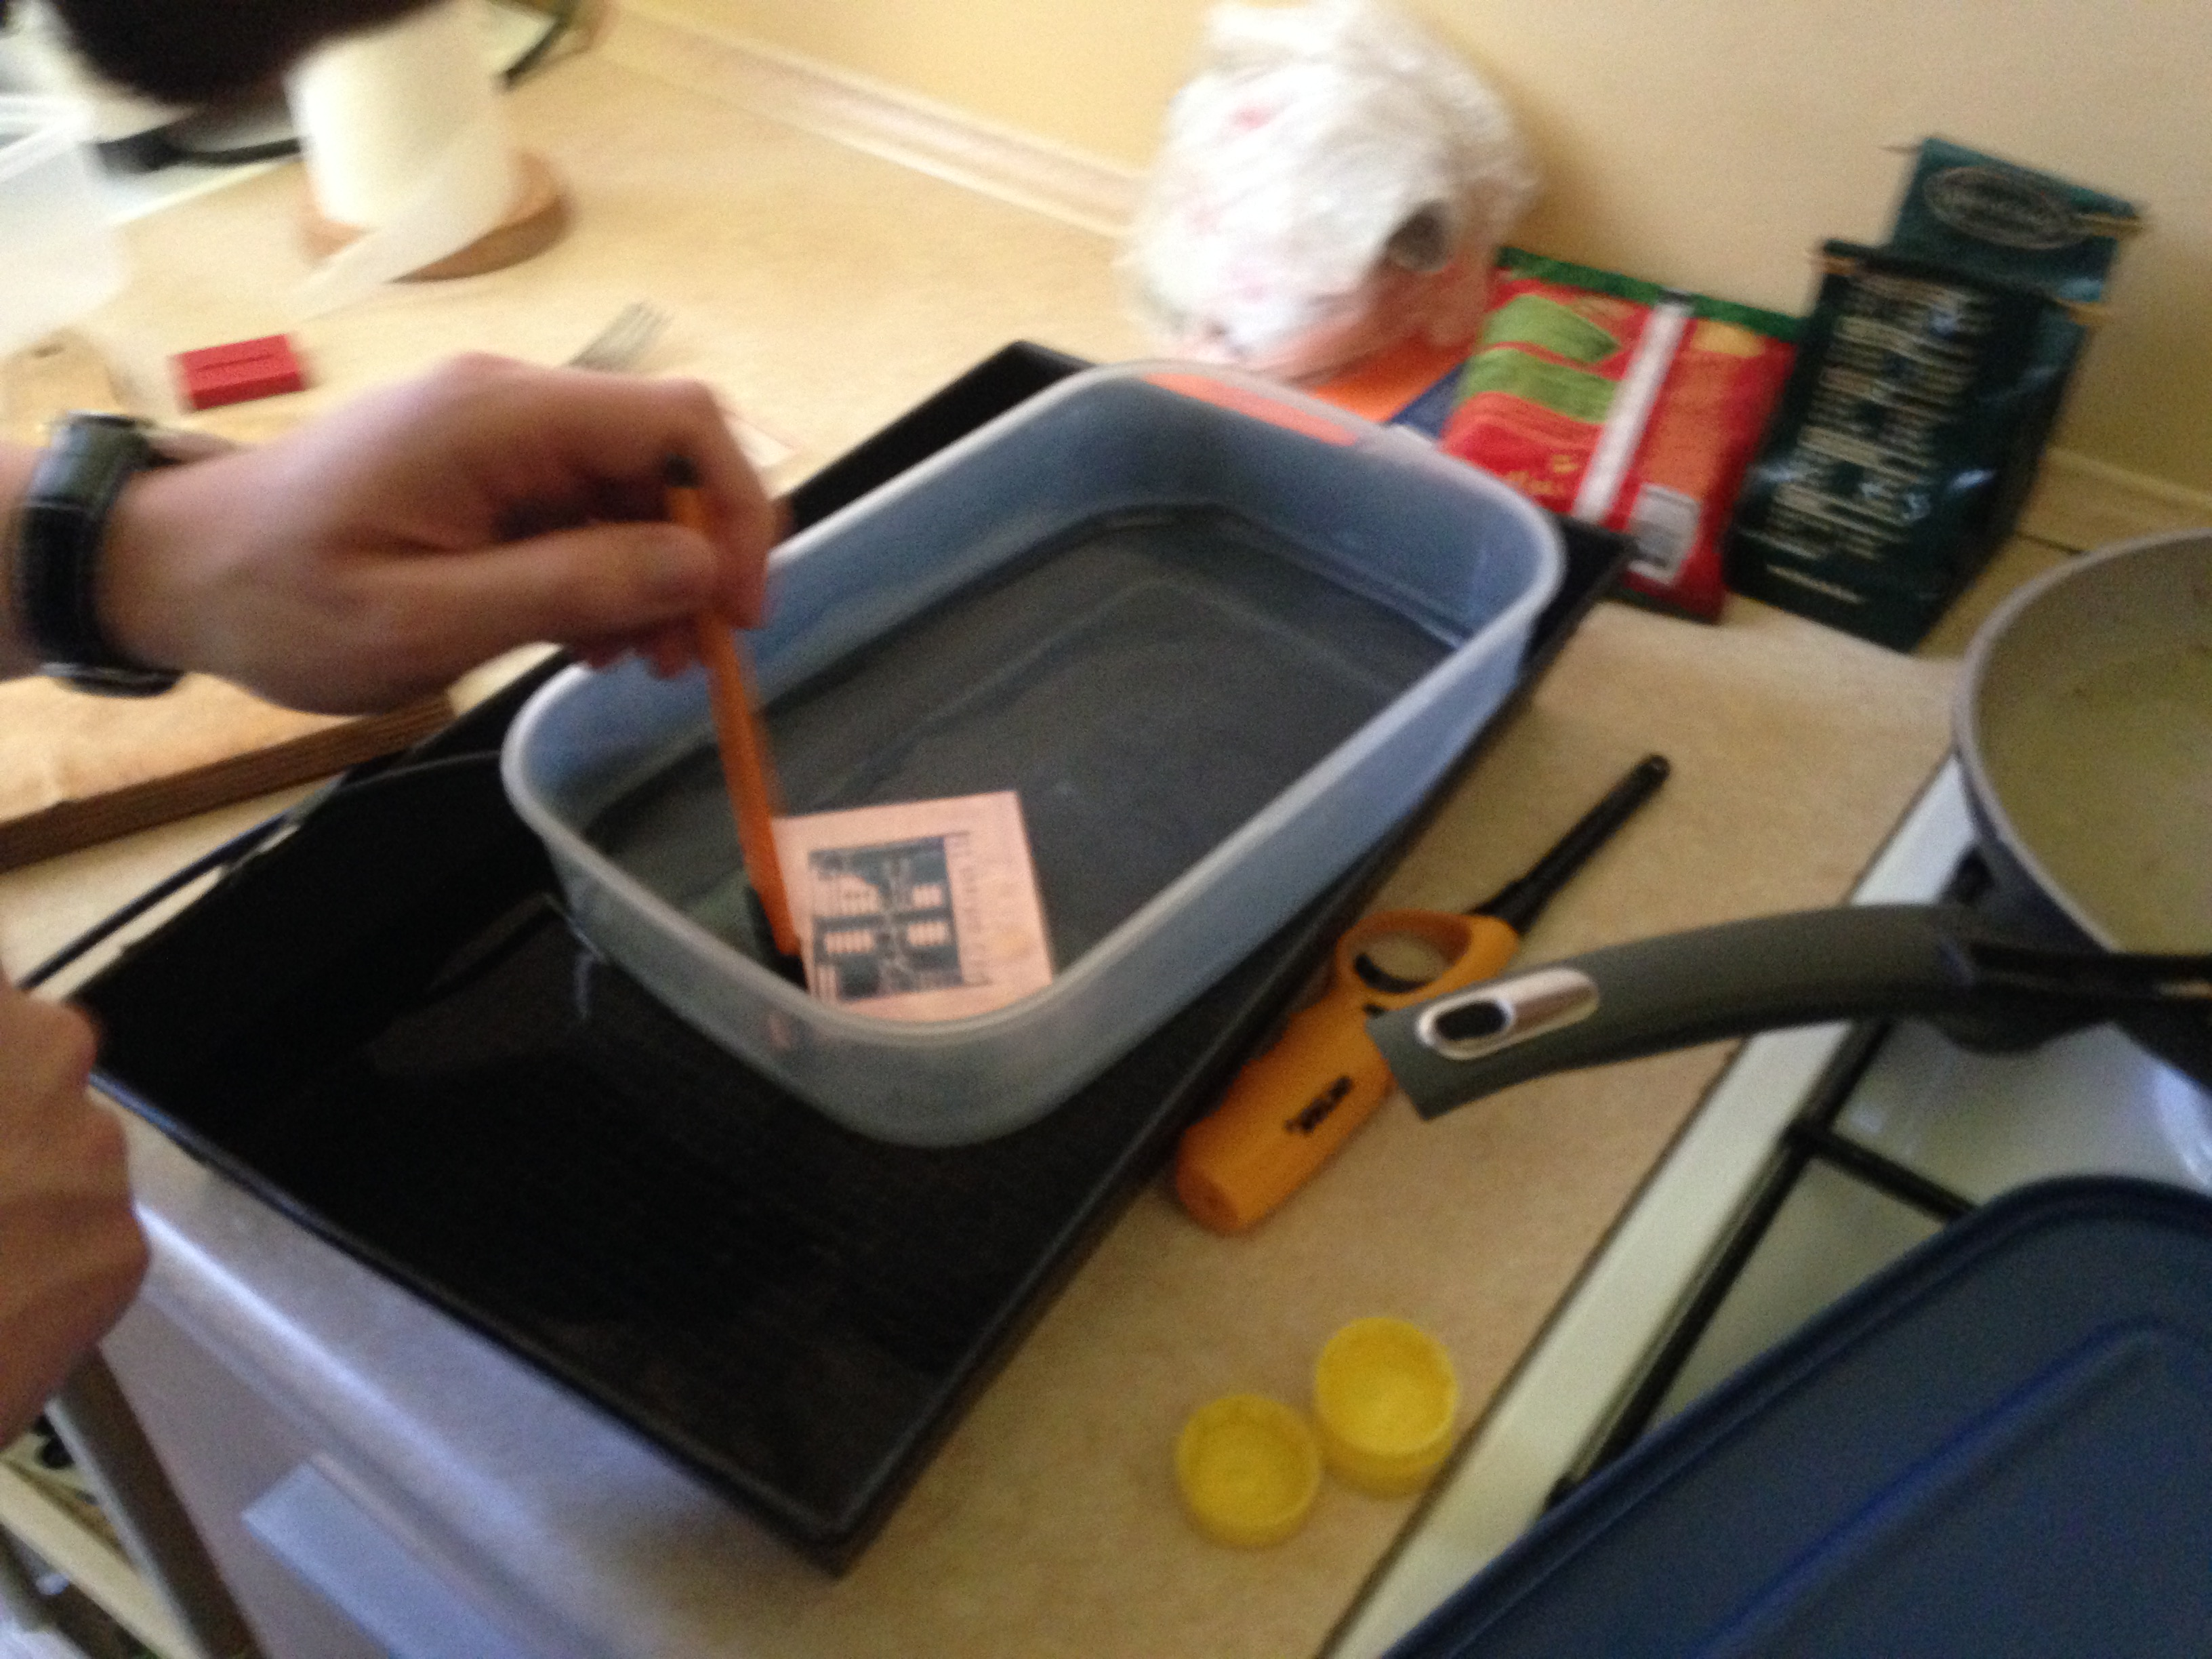
\includegraphics[width=\SCALE
	\paperwidth]{wanienka}
	\caption{prowizoryczna łaźnia laboratoryjna}
Przydatna może być lepsza izolacja naczynia zewnętrznego. Przedstawione naczynie dość szybko traci ciepło co wiąże się z dolewaniem dużych ilości ciepłej wody.
\end{figure}


Płytkę należy włożyć do roztworu i trzymać do zaniku miedzi nieprzykrytej tonerem. Trwa to ok 15. min. Poruszanie płytką lub mieszanie w roztworze ułatwi wytrawianie miedzi. Zbyt długie trzymanie płytki w roztworze spowoduje podtrawianie ścieżek i w konsekwencji ich przerwanie.

\subsection{Wiercenie}
W wytrawionej płytce należy wywiercić otwory montażowe. W tym celu należy użyć wiertła 1mm. Aby wiertło nie ślizgało się po płytce można zrobić małe dziurki śrubką lub gwoździem.

\subsection{Lutowanie}
Elementy należy przylutować do płytki. Zapewnia to dobre elektryczne połączenie jak i przytwierdza elementy do płytki. Można użyć zwykłej kolbowej lutownicy. W celu poprawy jakości i komfortu lutowanie można zastosować kalafonie, jednak nie jest to niezbędne. Są dostępne cyny z topnikiem który ma ułatwić lutowanie.

\section{Program}

Program działa jak regulator PID. Jednak z częścią całkującą pojawiły się pewne problemy dlatego czasem dobrze jest jest ograniczyć go do sterownika PI.

\lstinputlisting[language=C++]{../FTL.ino}

\section{Serwisowanie i konserwacja}
Regularnego przeglądu wymagają czujniki. Robota wyposażyliśmy w system do ich regulacji. Wystarczą do tego obcęgi. Należy robota utrzymywać możliwie blisko trasy, ale tak by koła jej nie dotykały. Każdy z czujników na swojej wierzchniej stronie posiada czerwoną diodę LED, które poinformuje nas czy czujnik poprawnie wykrywa linię. Ważną kwestią jest grubość linii. Najlepsze wyniki uzyskaliśmy dla około 2.0cm. Aktualnie robot jest ustawiony na 1.5cm, które było na RoboDayu. Im szersza linia tym szerzej należy rozstawić trzy wewnętrzne czujniki.

Baterie należy wymieniać po około 2 motogodzinach. Zalecamy wybór baterii alkaicznych AA o napięciu 1.5V - popularne "paluszki". Do pojemnika wchodzi 6 takich baterii i wszystkie są wymagane do poprawnej pracy silników i elektroniki. Silniki i elektronika są zasilane z jednego źródła i nie wykazaliśmy zakłóceń tym spowodowanych.

\end{document}
